\chapter{Object reconstruction}
\label{chap:objects}

In this chapter the reconstruction of the physics objects necessary for performing searches with taus 
in the final state with \ac{CMS} will be discussed. Section \ref{sec:objects_pv} details the algorithms
used to reconstruct charged particle tracks in the inner tracker, with section \ref{sec:objects_ele}
describing how these tracks are combined with \ac{ECAL} energy deposits to reconstruct electrons.
The reconstruction of muons by the combination of tracks in the inner tracker with hits in the muon 
chambers will be discussed in section \ref{sec:objects_muo}.
Section \ref{sec:objects_pf}
describes the \ac{PF} algorithm, which uses information from all sub-detectors in \ac{CMS} to reconstruct
all stable particles. \ac{PF} is of particular importance for the reconstruction of jets, missing transverse
energy and hadronically decaying taus as detailed in sections \ref{sec:objects_jets}, \ref{sec:objects_met} and \ref{sec:objects_tau} 
respectively.

\section{Tracks and vertices}
\label{sec:objects_pv}
To reconstruct the trajectories of charged particles, and therefore
their momenta and positions, from the hits they leave in the 
inner tracker the
\ac{CTF} algorithm is used \cite{cms-trk-algos}. This algorithm performs four steps.
First, initial estimates of the parameters of the trajectory are given by track seeds, 
made out of the hits found in two or three layers of the inner tracker. These track seeds
are extrapolated using a \ac{KF} \cite{trk-kf}, which extrapolates the seeding
trajectories along the expected flight path of a charged particle. Any additional
matched hits found along this extrapolated trajectory are added to the track.
After the extrapolation has reached the final tracker layers the \ac{KF} is run again,
now with the full set of hits that have been found in the previous step. This provides the best
estimate of the track parameters. Finally, tracks that fail a set of quality 
criteria are rejected.

These four steps are repeated six times. After each iteration
the hits associated with reconstructed tracks are removed and the settings
of the algorithm updated, in order to reconstruct as many
tracks as possible. The tracking efficiency for muons and pions was measured in p-p
collisions at $\sqrt{s} = 7\,\TeV$ and found to be $ > 98.5\%$ for tracks
with $\pTm > 500\,\MeV$ and $ > 99 \%$ for tracks with $\pTm > 2\,\GeV$ \cite{cms-trk-7tev}.
%The tracking software at CMS is commonly referred to as the Combinatorial Track Finder (CTF), which is an adaptation of the combinatorial Kalman filter [29–31], which in turn is an extension of the Kalman filter [32] to allow pattern recognition and track fitting to occur in the same frame- work. The collection of reconstructed tracks is produced by multiple passes (iterations) of the CTF track reconstruction sequence, in a process called iterative tracking.
%Kalman filter : In its linear form the Kal- ,nan filter is the optimal recursive estimator of the state vector of a (discrete) linear dynamic system. In such a system the evolution of the state vector is described by a linear transformation plus a random disturbance w, which is the process noise

\enlargethispage{\baselineskip}
Primary vertices are reconstructed by clustering
tracks that are compatible with having originated from the same vertex, then fitting 
these tracks for the position of the vertex. The clustering 
is performed using the \ac{DA} algorithm \cite{vtx-da}, which identifies
the most probable vertex candidates and assigns tracks to them. Vertex
candidates with at least two associated tracks are fitted using an adaptive
vertex fitter \cite{vtx-adaptivefit} to determine the best estimate of the 
vertex position. The \Htohhtobbtautau and \AHtotautau analyses, described in chapters \ref{chap:hhh} and \ref{chap:mssm},
take the primary
vertex of the hard scatter to be the reconstructed vertex with the largest scalar \pT~sum of the associated
tracks. %which the scalar sum of the \pT s of
%the associated tracks is largest. %This differs from the analysis presented in chapter \ref{chap:hhh},
%where requirements on the quality of the vertex
%fit and the distance between the vertex and the nominal interaction point 
%were additionally made.
 %By doing this both the best estimate
%of the vertex position and an indicator for the success of the fit are obtained.
%Each track is assigned a weight $w_i$ between 0 and 1, where values 
%closer to 1 indicate more consistency with the vertex position.
%The number of degrees of freedom in the fit can then be defined as
%\begin{equation}\label{eqn:pv_ndof}
%n_{\text{dof}} = -3 + 2 \Sigma_{i=1}^{Ntracks}w_i,
%\end{equation}
%which is strongly correlated with the number of tracks arising from the interaction region
%and can therefore be used to select genuine interactions. During Run 1 this variable was
%used in many analyses, including the one presented in chapter \ref{chap:hhh}, to define
%good--quality primary vertices. In addition to requiring $n_{\text{dof}}>4$, the distances
%between the vertex and the nominal interaction point were required
%to be $\Delta z< 24$ cm and $\Delta xy < 2$ cm. The primary vertex of the
%hard scatter was then taken as the vertex with greatest scalar sum \pT~ of associated
%tracks that passed these requirements. For the analyses with data from Run 2 the
%quality requirements were removed and the primary vertex of the hard scatter was simply taken
%as the reconstructed vertex with largest scalar sum \pT~ of tracks.

The resolutions of the $x$ and $z$ coordinates of the primary vertex were measured in
collisions at $\sqrt{s}=13\,\TeV$ and depend strongly on the number of tracks
associated with the vertex, as figure \ref{fig:objects_tracks_pvres} shows.
~\vspace{-1\baselineskip}
\begin{figure}[h!]
\begin{center}
\subfloat[Resolution in x]{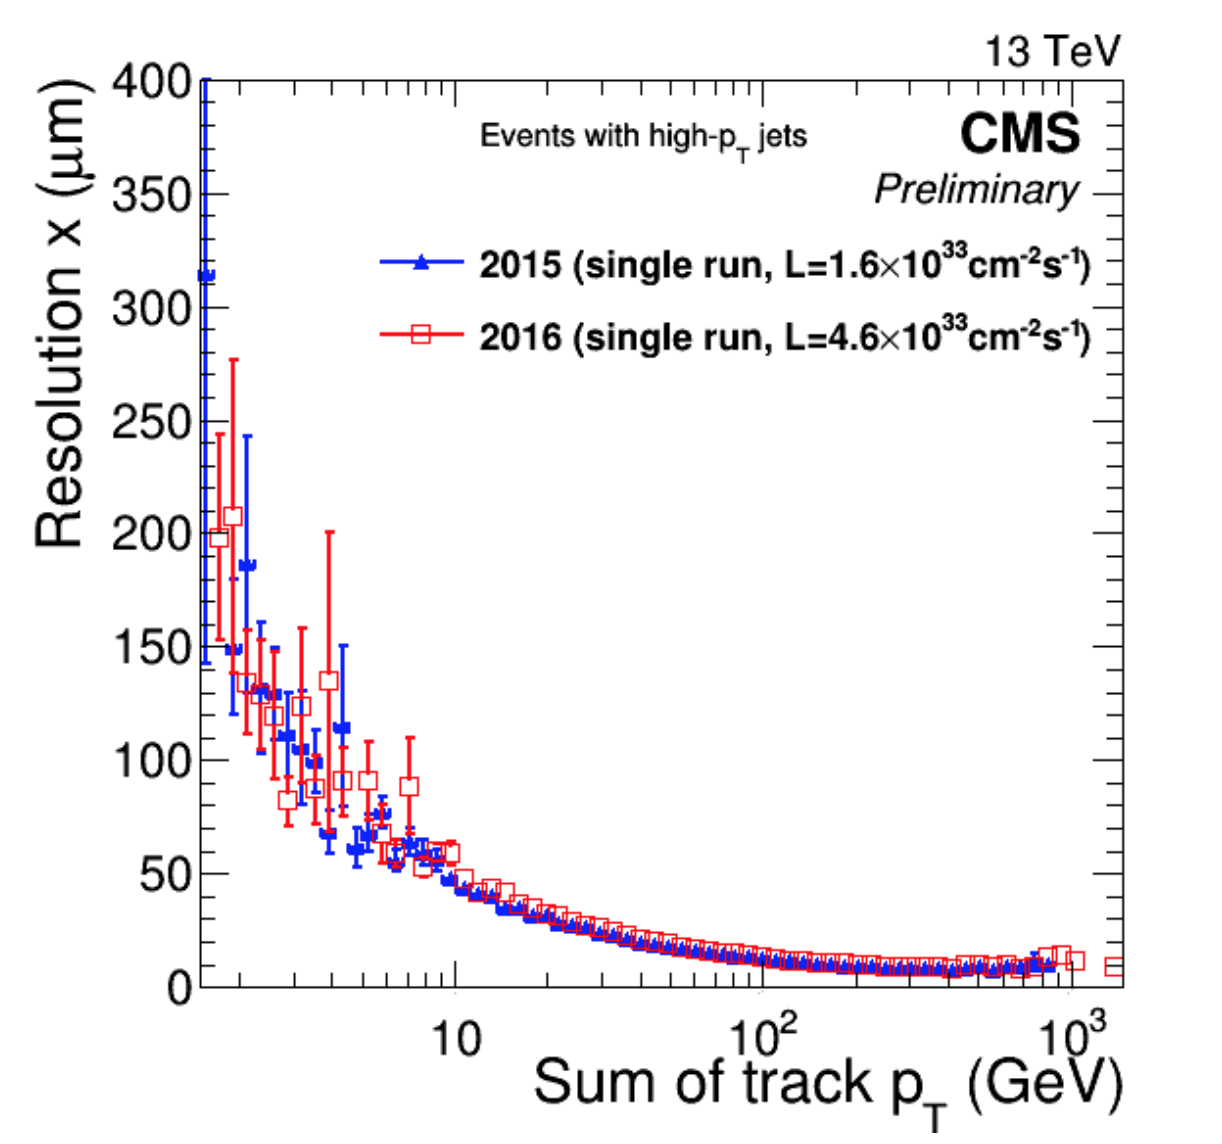
\includegraphics[width=0.5\textwidth]{./Objects/Plots/PVResX.png}}
\subfloat[Resolution in z]{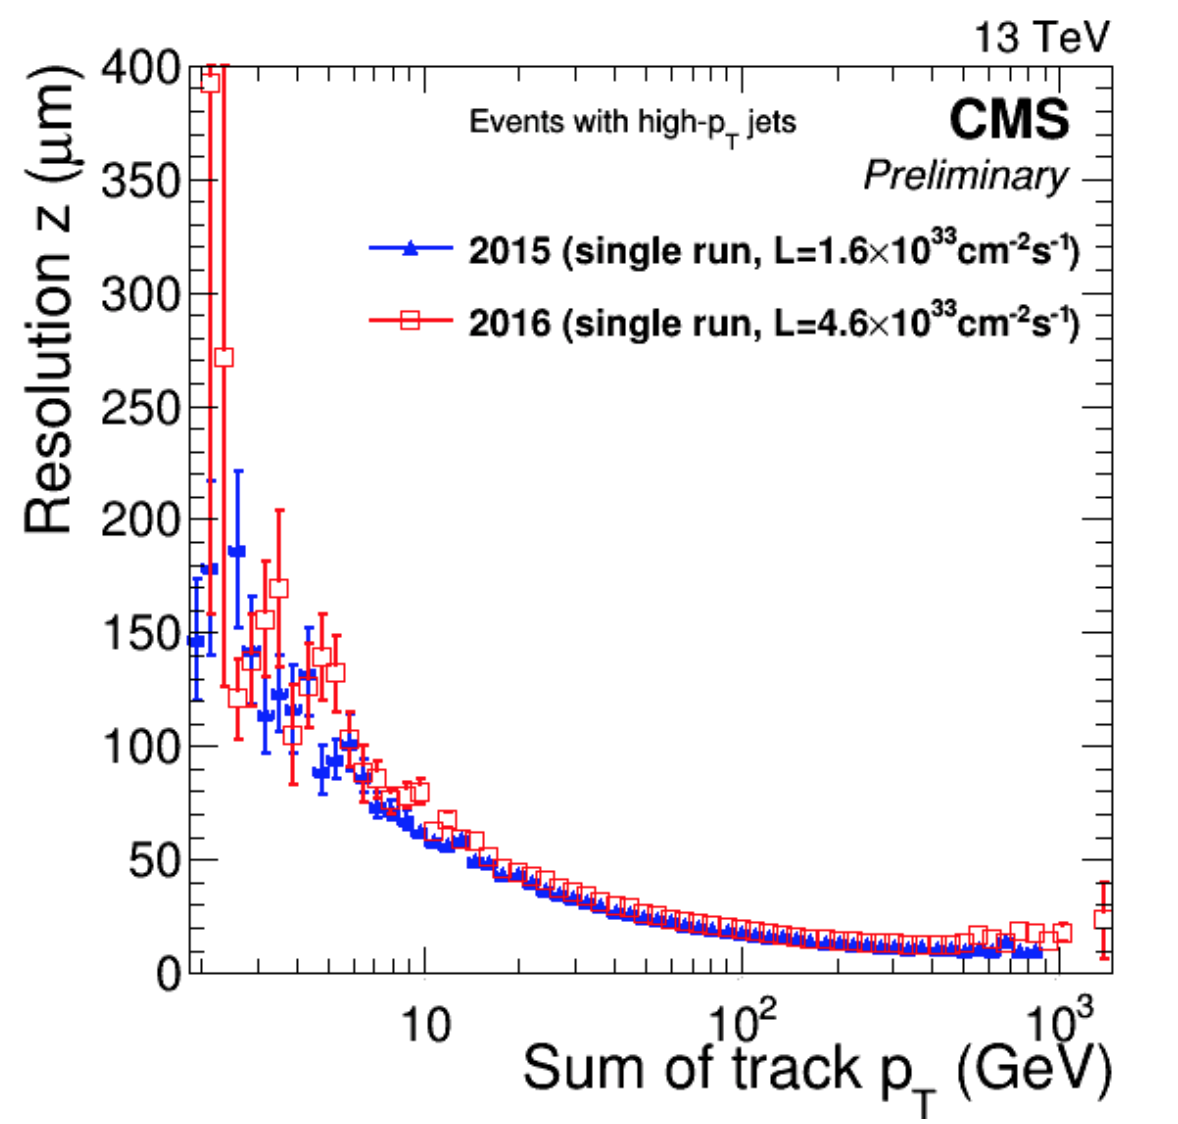
\includegraphics[width=0.5\textwidth]{./Objects/Plots/PVResZ.png}}
\end{center}
\caption[Resolution of the $x$ and $z$ coordinates of reconstructed
primary vertices as a function of the scalar \pT~sum of the associated
tracks.]{Resolution of (a) the $x$ coordinate and (b) the $z$ coordinate 
of reconstructed primary vertices
as a function of the scalar \pT~sum of the associated tracks, 
measured in 2015 (blue triangles) and 2016 (red squares).
The resolution improves
with higher scalar \pT~sum of the associated tracks, which corresponds to larger numbers of tracks \cite{cms-trk-dp}.}
\label{fig:objects_tracks_pvres}
\end{figure}


\section{Electrons}
\label{sec:objects_ele}
Electrons are reconstructed by combining tracks from 
the inner tracker with energy deposits in the \ac{ECAL}.
A standalone electron reconstruction algorithm \cite{cms-elereco-run1} complements the \ac{PF} approach
that will be described in section \ref{sec:objects_pf}. %FIXME don't say this, they're more similar now
Depending on the thickness of the intervening material, electrons lose up to an average of 86\% of their energy 
due to bremsstrahlung before reaching the \ac{ECAL}.
To accurately reconstruct the energy of the electron it is
important to capture the energy of the bremsstrahlung photons, which are spread in the $\phi$ direction
due to the magnetic field. To achieve this, ``supercluster'' algorithms are used.
In these algorithms the clustering
is performed by defining a seed crystal as the crystal containing a local
energy maximum above a certain threshold.
In the barrel, arrays of $5\times 1$ crystals in $\eta \times \phi$ are then added
to the cluster, stepping sideways in both directions in $\phi$ within a range
of approximately $\pm 0.3$ rad. Contiguous clusters are merged into
superclusters as long as each cluster satisfies a minimum energy deposit.
In the endcaps arrays of $5\times 5$ crystals are 
merged into superclusters within a range in $\eta$ of $\pm 0.07$ and a range in $\phi$ of $\pm 0.3$ rad.
%The array is
%only added to the cluster if the energy deposited in it is larger than a minimum.
%These clusters are grouped into superclusters if each distinct cluster has a seed array in 
%which the energy deposit is larger than a pre-defined minimum.

Due to the radiation of bremsstrahlung photons in the tracker,
the change in curvature of the electron track can be large. % and so the \ac{CTF} does
%not perform optimally. 
Therefore a dedicated tracking algorithm is used, with better performance than the \ac{CTF} for this 
particular case.
For high-\pT~electrons the best efficiency is reached
by the use of an \ac{ECAL}-based track seeding algorithm \cite{cms-elereco-run1}.
This algorithm extrapolates the position and energy of the supercluster to the first
layers of the tracker to determine the approximate area where the tracker seeds should be.
Once the tracker seeds have been found they are extrapolated
and smoothed using the \ac{GSF} \cite{trk-gsf} instead of the \ac{KF}, which 
approximates the non-Gaussian energy loss in each layer by a combination of 
Gaussian distributions rather than the single Gaussian used in the \ac{KF}.

%Once the hits are collected, a GSF fit is performed to estimate the track parameters. The energy loss in each layer is approximated by a mixture of Gaussian distributions. A weight is at- tributed to each Gaussian distribution that describes the associated probability. Two estimates of track properties are usually exploited at each measurement point that correspond either to the weighted mean of all the components, or to their most probable value (mode).

For a particle to be identified as an electron it 
must also be reconstructed as an electron by the \ac{PF} algorithm, 
and must in addition pass more advanced identification criteria based on some of the variables used in the
standalone electron reconstruction. This provides separation power from backgrounds
such as photon conversions, jets misidentified as electrons, or electrons from b- and c-quark
decays. Both a cut-based algorithm and an algorithm based on \acp{BDT} are available. %FIXME define BDT
For the selection of electrons in 
the analyses presented in later chapters the \ac{BDT}-based algorithm is used, 
with exceptions for the loose identification criteria required for vetoing electrons. 
The variables used in this \ac{BDT} include:%FIXME full stop usage?!
\begin{itemize}
\setlength{\itemsep}{-0.5\baselineskip}
\item Cluster shape variables, such as $\sigma_{i\eta,i\eta}$, the energy-weighted width of the supercluster in units of $\eta$ crystals (illustrated in figure \ref{fig:ele_id_vars}a). 
\item Track quality variables.
\item Distances in $\eta$ and $\phi$ between the supercluster and the associated track.
\item Energy ratios and energy-momentum ratios in the region of the supercluster, including
$1/E_{\text{SC}} - 1/p_{\Pe}$, where $E_{\text{SC}}$ is the energy in the supercluster and $p_{\Pe}$ the momentum of the electron track (illustrated in figure \ref{fig:ele_id_vars}b).
%\item Cluster shape variables $\sigma_{i\eta,i\eta}$ and $\sigma_{i\phi,i\phi}$, with $i\eta$ and $i\phi$ the integer
%label of the $\eta$ and $\phi$ calorimeter cell. The circularity =  $1 -\frac{E1\times5}{E5\times5}$, with
%$E1\times5$ and $E5\times5$ the energies in a $1\times5$ and a $5\times5$ grid around the super cluster seed,
%respectively. Shape variable R9 = $\frac{E3\times3}{E_{SC}}$, with $E3\times3$ the energy in a $3\times3$ grid
%of cells around the super cluster seed and $E_{SC}$ the raw energy of the super cluster.
%\item The number of valid hits in the track fit, the $\chi^2$ of the track fit and the $\chi^2$ of the GSFTrack fit
%%\item The number of GSFtrack hits, the number of expected missing inner hits and the result of the conversion vertex fit
%\item The distance $\Delta \eta$ and $\Delta \phi$ between the reconstructed super cluster and the associated track at the position of the primary vertex, and the distance in $\eta$ between the super cluster and the track at the calorimeter surface.
%\item H/E, the ratio of the hadronic energy over the electromagnetic energy in the super cluster and E/P, the ratio of the super cluster energy over the momentum of the track associated with the electron
%\item The ratio of the energy of the electron cluster and the momentum of the associated track, evaluated at the electron cluster,
% and $1/E_e - 1/P_e$, with $E_e$ the energy of the electron candidate and $P_e$ its momentum.
\end{itemize}
%Figure \ref{fig:ele_id_vars} shows the distributions of $\sigma_{i\eta,i\eta}$ and $1/E_{sc} - 1/p_e$ 
%for real and misidentified electrons in the full dataset from the 2012 running period of the \ac{LHC}.

\begin{figure}[h!]
\begin{center}
\subfloat[$\sigma_{i\eta,i\eta}$]{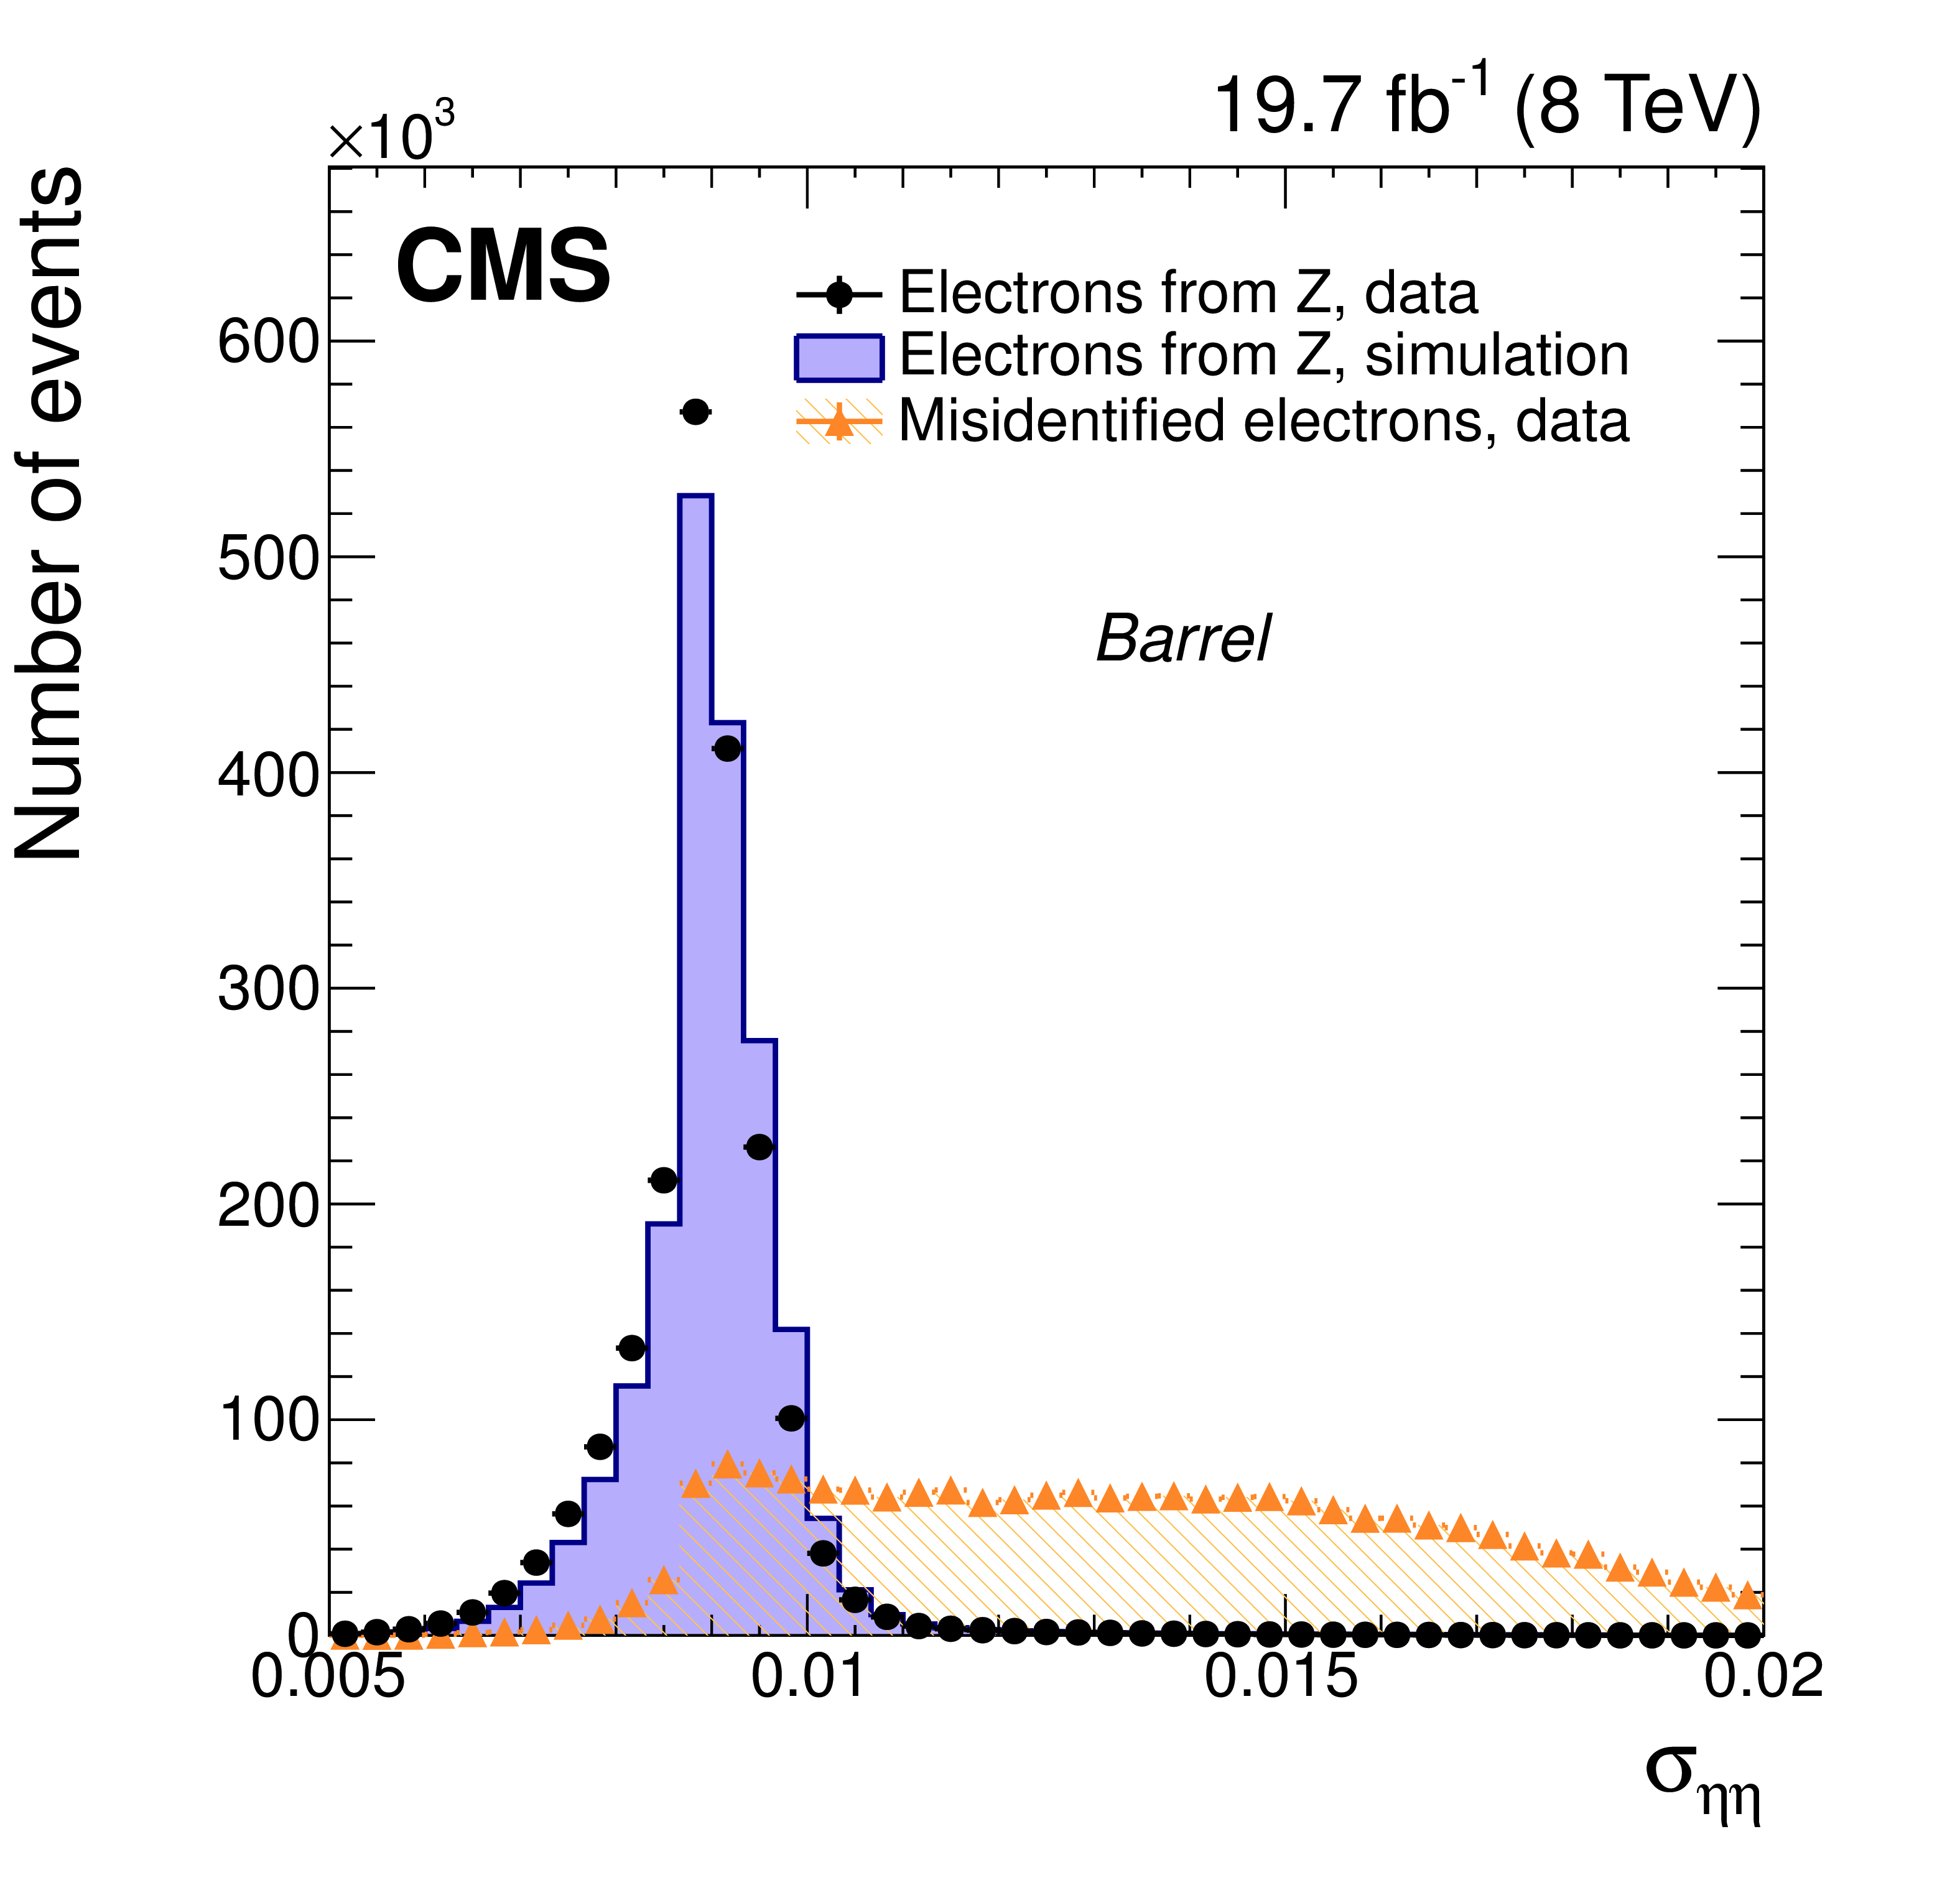
\includegraphics[width=0.5\textwidth]{./Objects/Plots/Sigmaietaieta.png}}
\subfloat[$1/E_{\text{SC}} - 1/p_{e}$]{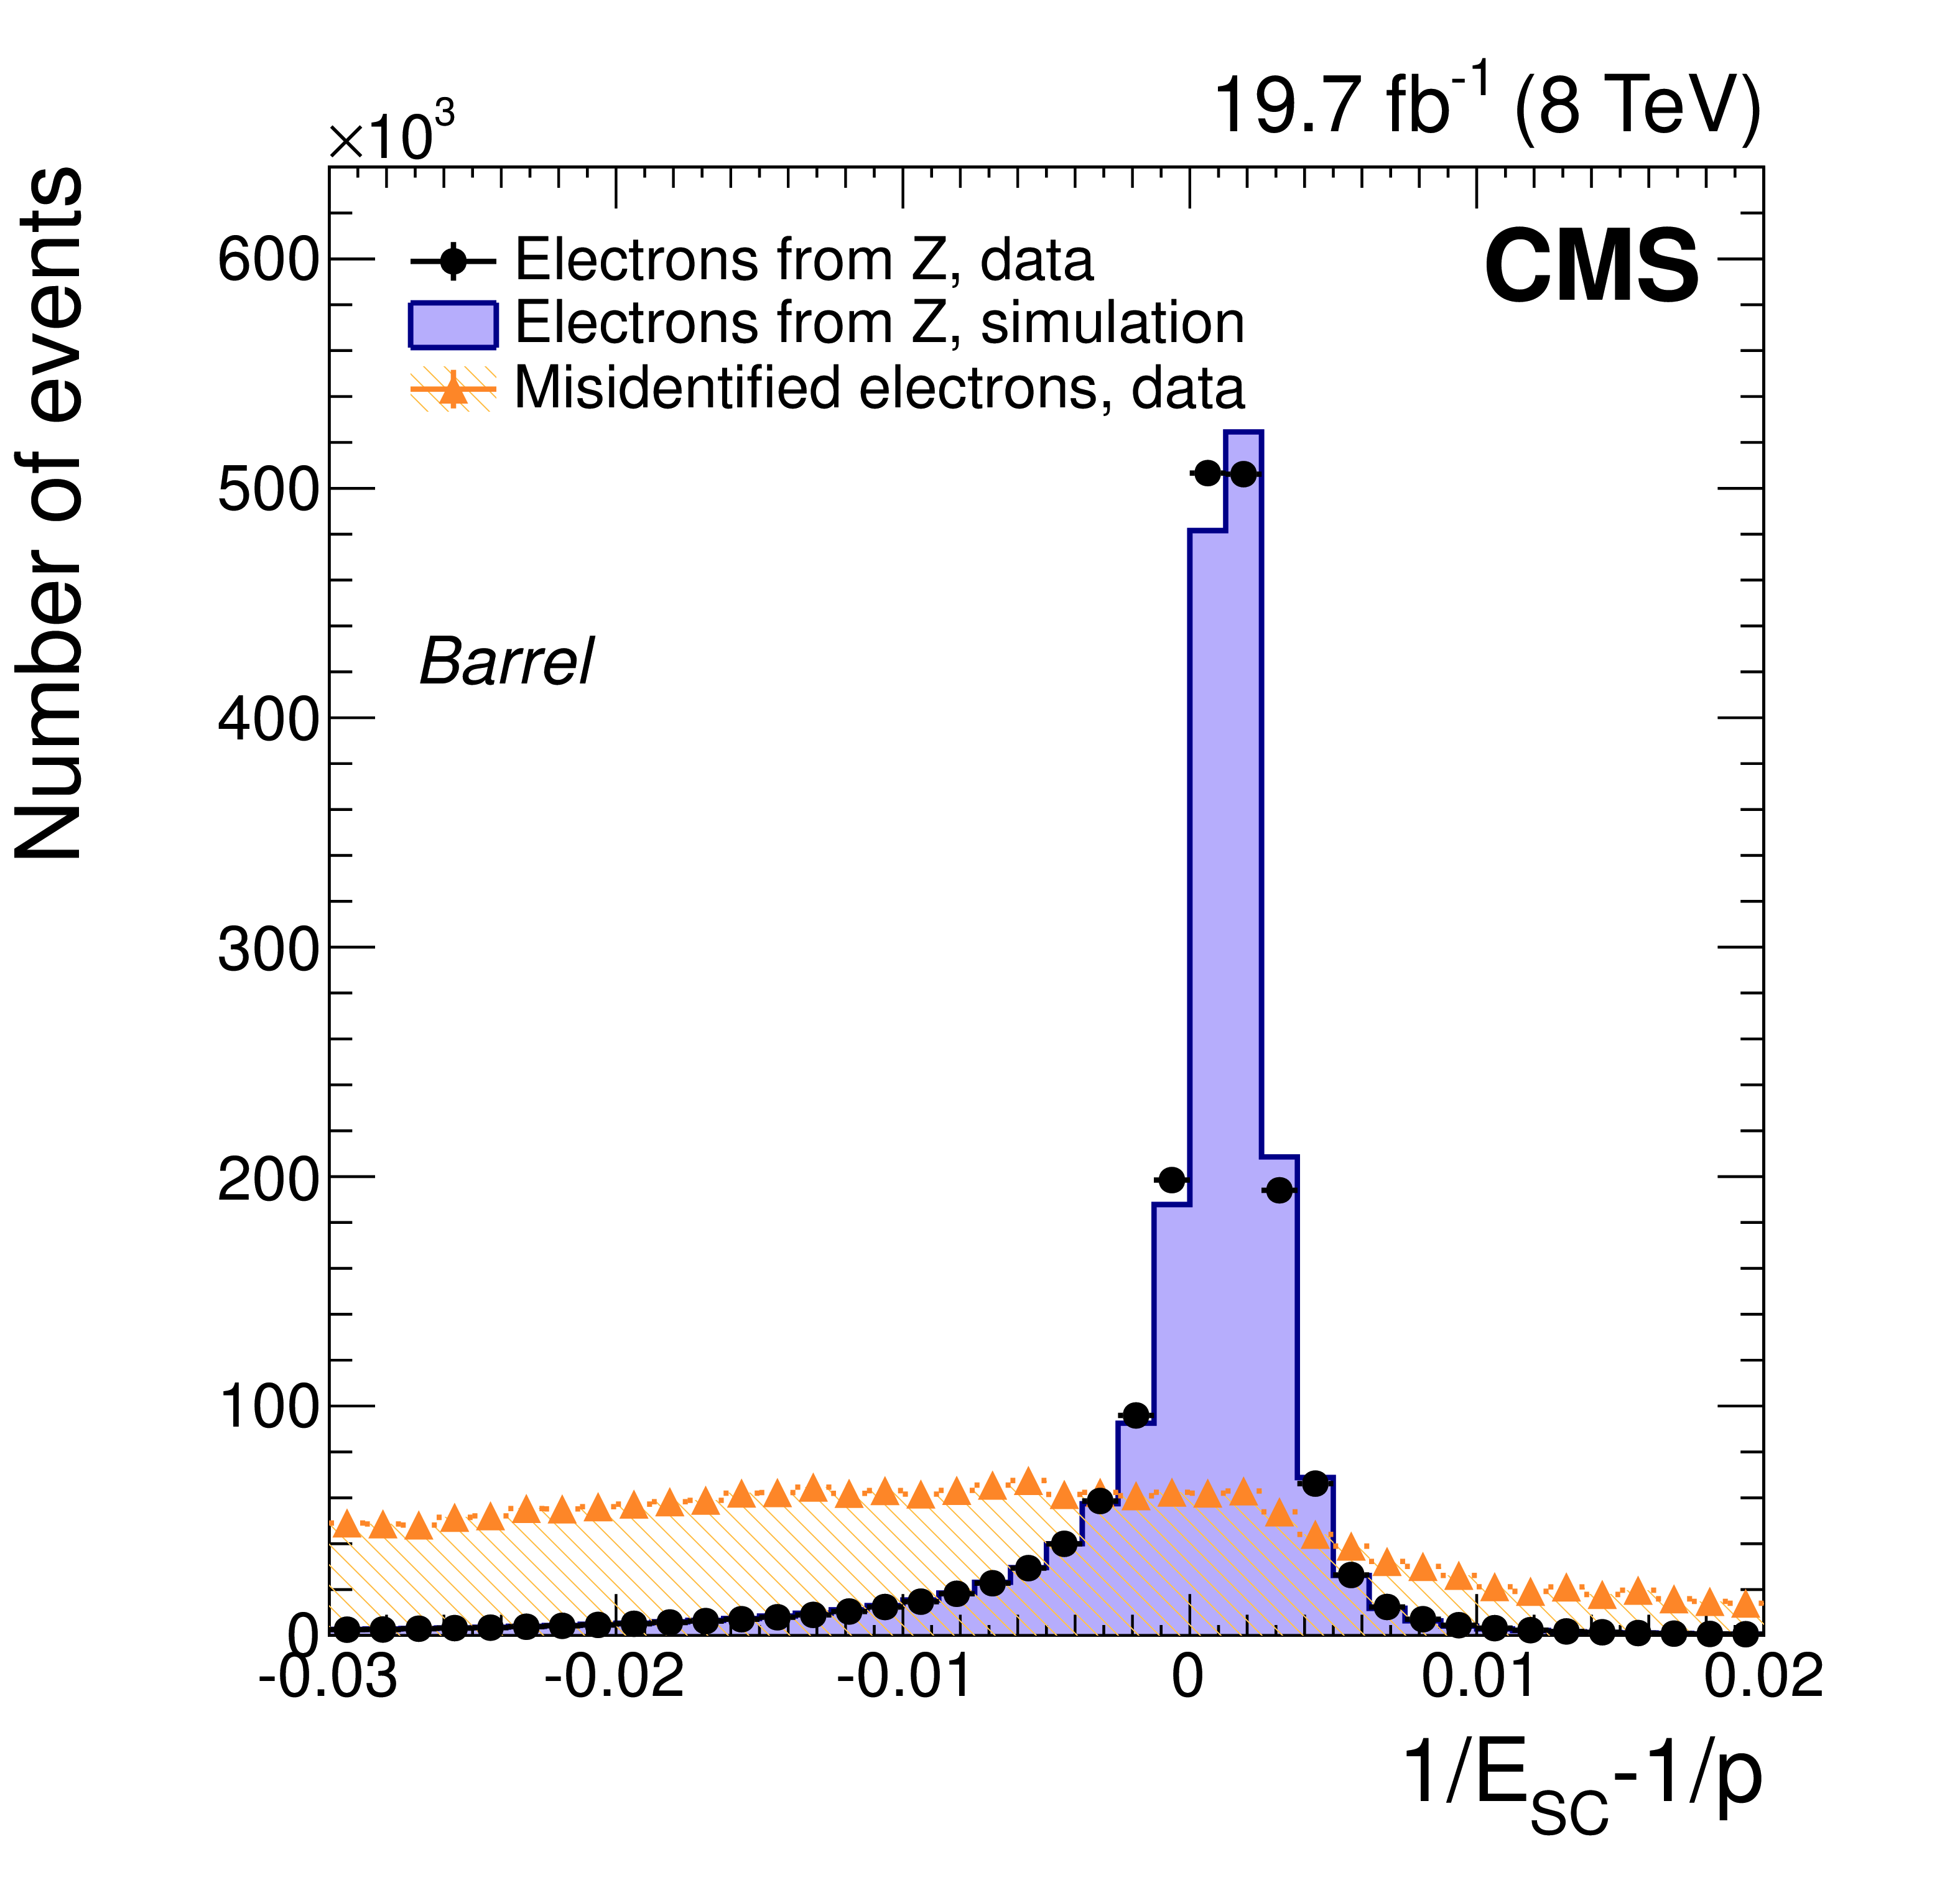
\includegraphics[width=0.5\textwidth]{./Objects/Plots/OneoverEminOneoverp.png}}
\end{center}
\caption[$\sigma_{i\eta,i\eta}$ and $1/E_{\text{SC}}-1/p_{e}$ for real 
and misidentified electrons at $8\,\TeV$, for data and simulation.]{(a) $\sigma_{i\eta,i\eta}$ and (b) $1/E_{\text{SC}} - 1/p_{e}$ for real (black points)  and 
misidentified (yellow triangles) electrons in a dataset corresponding to $19.7\,\invfb$
taken at $\sqrt{s} = 8\,\TeV$, overlaid on the distributions for simulated 
real electrons in purple \cite{cms-elereco-run1}.}
\label{fig:ele_id_vars}
\end{figure}

%\subsection{Isolation}
%\label{sec:objects_ele_iso}
The identification requirements discussed up to now reduce the backgrounds 
from misidentified electrons, but do not eliminate them completely. If jets are
misidentified as electrons, or an electron resulting from a heavy-flavour 
decay is identified, the electron is not isolated. Therefore requirements
on the electron isolation can reduce these backgrounds even further.
Different isolation definitions are used in \ac{CMS}. The default, which is
used for the analyses presented in later chapters, is a combined relative isolation variable
defined as \cite{SMHtautauCMS}:
\begin{equation}\label{eqn:electron_reliso}
I_{\text{rel}} = \frac{\Sigma p_{\text{T}}^{\text{charged}} + \mathrm{max}(\Sigma E_{\text{T}}^{\text{neutral}} + \Sigma E_{\text{T}}^{\text{photon}} - \Delta\beta \Sigma E_{\text{T}}^{\text{PU}},0)}{p_{\text{T}}^{e}},
\end{equation}
where the \pT~and \ET~sums are taken within a cone in $\eta$-$\phi$ around the direction
of the electron of size $\Delta R = 0.4$ during Run 1 and $\Delta R = 0.3$ during Run 2 \cite{CMS-PAS-HIG-16-037}.
The sum over \pT$^{\text{charged}}$ corresponds to the \pT~of all charged %\ac{PF} 
hadrons associated with the primary vertex. %and within the cone of radius $\Delta R$ around
%the electron's axis. 
The \ET$^{\text{neutral}}$ and \ET$^{\text{photon}}$ sums
run over all neutral hadronic energy and photon energy. %within the cone of radius $\Delta R$.
The contribution from neutral particles due to pileup needs to be subtracted from
the sum of these two terms. It is estimated as the sum of charged hadronic \pT~for hadrons not associated
with the primary vertex, multiplied by a $\Delta \beta$ factor of $\frac{1}{2}$.

\section{Muons}
\label{sec:objects_muo}
Muons are reconstructed by combining tracks in the inner tracker with tracks
from the muon system \cite{cms-muon-reco}. Two complementary approaches are used:
``global'' and ``tracker'' muon reconstruction. The former starts from 
tracks reconstructed in the muon system and searches for a matching
tracker track, then reapplies the \ac{KF} to the combination
of hits in the muon system and inner tracker. Conversely, the tracker muon reconstruction starts from
tracks in the inner tracker which pass requirements on \pT~to be considered
a muon candidate track. The trajectory is then extrapolated to the muon systems and
considered a muon if at least one muon segment, a track stub in the \acp{DT} or \acp{CSC}, is found.
Due to the requirement of a single muon segment this method is more efficient than the global muon
reconstruction for muons with \pT~smaller than $5\,\GeV$ \cite{cms-muon-reco}.
For muons with \pT~greater than $200\,\GeV$, the momentum resolution is improved
by the global muon reconstruction \cite{cms-muon-cosmics-perf}.

The muon momentum resolution was measured in p-p collisions at $\sqrt{s}=7\,\TeV$ 
for muons with \pT~up to $100\,\GeV$ and found to range from 1--6\% depending
on detector region. For muons with \pT~between $100\,\GeV$ and $1\,\TeV$ the momentum resolution
was determined to be better than 10\% in the barrel region using cosmic rays \cite{cms-muon-reco}.
%At values of the transverse momentum pT below about 200 GeV/c, the momentum resolution for a muon track is driven by measurements in the silicon tracker. As a particle’s momen- tum increases and the curvature of its corresponding track decreases, however, momentum resolution in the tracker becomes limited by position measurement resolution (including mis- alignment effects). One can then benefit from the large lever arm and 3.8 T magnetic field in the region between the tracker and the muon system by including hits in the muon chambers.

For global muon reconstruction the non-muon backgrounds are small,
though there can be a small contamination from hadronic showers not fully
contained in the \ac{HCAL}. A larger contribution is expected
from real muons originating from, for example, decays of hadrons. These
backgrounds can be reduced by applying additional identification criteria.

For the \AHtotautau analysis, ``medium'' muon requirements were applied \cite{CMS-PAS-HIG-16-037}.
These requirements include:
\begin{itemize}
\setlength{\itemsep}{-0.5\baselineskip}
\item Reconstruction by either the global or tracker muon reconstruction algorithms.
\item Requirements on track quality, and compatibility between the tracker track and the muon system track.
\item Selection on the segment compatibility, a weight between 0 and 1 which is a measure of the compatibility
of a track with the muon track segments in the muon stations it has crossed.
\item Requirements on the maximum kink in the tracker track in any of the layers of the tracker, to suppress in-flight decays.
\end{itemize}
%Apart from having passed either the global or tracker muon reconstruction, the selection
%includes a threshold on the fraction of valid tracker hits, requirements on the
%$\chi^2$/$N_{\text{dof}}$ of the global track fit, on the compatibility of the tracker- and standalone-reconstructed
%position matching, on the kink finder in the inner tracker, and the segment compatibility. 
%The compatibility of the tracker- and standalone-reconstructed position is evaluated
%by extrapolating both the muon track and the tracker track to the same surface and evaluating the $\chi^2$ 
%compatibility there.
%The kink finder determines the $\chi^2$ compatibility between the positions of the outward- and inward interpolated
%tracks in each layer of the inner tracker. The largest $\chi^2$ value found at any of the tracker layers 
%is used as a discriminator. If the $\chi^2$ value is large, this could signal an in--flight decay.
%The segment
%compatibility is a weight between 0 and 1 which is a measure of the compatibility of a track with
%the muon track segments in muon stations it has crossed. Numbers closer to 1 represent
%a greater compatibility of the track with the muon segments, and therefore with the track belonging to a muon.
%MEDIUM REQUIREMENTS
%To pass the identification, global- or tracker muons
%with a large enough fraction of tracker hits must pass \textbf{either} 
%\begin{itemize}
%\setlength{\itemsep}{-\baselineskip}
%\item The muon is reconstructed by the global muon reconstruction algorithm
%\item The $\chi^2$/$N_{\text{dof}}$ of the global track fit, using both the tracker and muon system hits, should be less than 3
%\item The $\chi^2$ compatibility of the tracker-standalone position is smaller than 12
%\item The $\chi^2$ compatibility of the kink finder in the tracker is less than 20
%\item The segment compatibility is $>$ 0.303
%\end{itemize}
%\textit{or}:
%\begin{itemize}
%\setlength{\itemsep}{-\baselineskip}
%\item The segment compatibility is $>$ 0.451
%\end{itemize}

In the \Htohhtobbtautau analysis, where Run 1 data 
was used, muons were required to pass ``tight'' identification requirements \cite{cms-muon-reco}. 
In addition to having to be reconstructed by the global muon algorithm, selections
are made on the $\chi^2$ per degrees of freedom of the track fit, number of hits of the inner
track in different tracker layers and number of muon segments the inner track is matched to.
%TIGHT REQUIREMENTS
%\begin{itemize}
%\setlength{\itemsep}{-\baselineskip}
%\item The muon must be reconstructed by the global muon algorithm
%\item The $\chi^2$/$N_{\text{dof}}$ of the global track fit must be smaller than 10
%\item The global track fit must include hits from at least one chamber in the muon system
%\item The inner tracker track must be matched to muon segments in at least two muon stations (which means the muon must also be reconstructed as a tracker muon)
%\item The tracker track must have at least one hit in the pixel detector, and hits in ten tracker layers.
%\end{itemize}

%\subsection{Isolation}
%\label{sec:objects_muo_iso}
As described for electrons in section \ref{sec:objects_ele}, placing isolation 
requirements on muons will also reduce backgrounds from misidentified jets and heavy-flavour
decays. The isolation variable used for muons is very similar to the one described for
electrons in equation \ref{eqn:electron_reliso}, however the cone around the direction of the
muon was chosen as $\Delta R = 0.4$ during both Run 1 and Run 2.

\section{Particle flow}
\label{sec:objects_pf}
All stable particles are reconstructed and identified using the \ac{PF} algorithm \cite{cms-pf-2009,cms-pf-2010-commfirst,cms-pf-2010-2}, which
combines the information from all of the different subdetectors of \ac{CMS}. This makes
the identification of particles, and determination of their position and momentum, as precise
as possible. All of these particles are then used to build, for example, jets, hadronically decaying taus and missing transverse
energy \MET, which will be discussed in subsequent sections.

The \ac{PF} algorithm starts from charged particle tracks measured
by the inner tracker, muon tracks measured in the muon system, and 
energy deposits in the calorimeters. These energy deposits are combined
using a clustering algorithm, so that stable neutral particles can be identified and
separated from charged hadrons, and in addition electrons and all bremsstrahlung photons
can be reconstructed. Clustering is performed separately in the \ac{ECAL} barrel,
\ac{ECAL} endcaps, first and second preshower layers, \ac{HCAL} barrel and \ac{HCAL} endcaps, with no 
clustering employed in the \ac{HF}.
%And to aid energy measurement of charged hadrons for which
%tracks were low quality, or high pT
The clustering algorithm used for \ac{PF} starts from cluster seeds,
calorimeter cells with local energy maxima. Topological clusters are built by 
merging neighbouring cells into the cluster, provided that the cells
being merged in contain a certain minimum energy.
The threshold is $800\,\MeV$ in the \ac{HCAL} and two standard deviations above the
expected noise level in the \ac{ECAL}, meaning $80\,\MeV$ in the barrel and up 
to $300\,\MeV$ in the endcaps. Cell energies can be shared between multiple
\ac{PF} clusters, depending on the distance between a cell and the centre of the cluster.

Any given particle will usually give rise to multiple \ac{PF}
elements in the different subdetectors. To provide full reconstruction
of each particle, and avoid double counting, the next step in the
\ac{PF} algorithm is to link the different elements. This is
achieved by defining a distance parameter between any two \ac{PF} elements
in the event, which quantifies the link quality. Directly and indirectly
linked elements are considered as input blocks to the reconstruction and
identification algorithm. Links between charged tracks and calorimeter
clusters are established by extrapolating the track from its last measured
tracker hit to the preshower layers, the \ac{ECAL} and the \ac{HCAL}. %in ECAL to expected maximum of a 
%typical longitudinal electron shower profile and in the HCAL at a depth correspnding to one interaction
%length.
If the extrapolated track position is within the boundaries of the cluster, plus the size
of one cell in each direction to account for gaps between cells and multiple scattering, the
track is said to be linked to the calorimeter cluster. The link distance parameter 
is taken as the distance $\Delta R$ 
between the position of the cluster and the position of the track. Tangents to tracks are also extrapolated
to the ECAL from the interaction points between the track and each tracker layer, and clusters can be 
linked to the track as a possible bremsstrahlung photon if the extrapolated tangent
position is within the boundaries of the cluster.
Links between calorimeter clusters are made when the cluster position in the
more granular calorimeter is within the cluster of the less granular calorimeter,
with the link distance again defined as the $\Delta R$ between the positions of the two clusters.
To determine links between charged tracks in the inner tracker and a muon track
in the muon system, a global fit between the two tracks is performed, where the link
is accepted if requirements on the maximum $\chi^2$ of this fit are met. This
$\chi^2$ also determines the distance parameter.

For each block, particles are identified following a sequence
of tests. Firstly, if there is a link between a tracker track and a muon system track,
a \ac{PF} muon is identified if the combined tracker and muon system
momentum is compatible with the tracker-only momentum. %within three standard deviations
The muon track is removed from the block before the next step of the algorithm.

Secondly, tracks are refitted with the \ac{GSF} and the compatibility
of the track with the already linked \ac{ECAL} clusters is assessed using
\acp{BDT} which take several variables into account. If the candidate
passes, it is identified as a \ac{PF} electron and the track and
\ac{ECAL} clusters are removed from the block.

After this, remaining tracks lead to charged hadrons. The track is
given the momentum from the track fit, assuming the mass of a charged pion. If
the energy measured in the calorimeters is compatible with the momentum assigned
to the track, a charged hadron is identified and the
momentum redefined by fitting the tracker and calorimeter measurements. If
the energy of the calorimeter clusters linked to the track is significantly larger than the
charged particle momentum from the track fit, additional overlapping neutral particles
are identified. If the difference between the tracker momentum and the calorimeter
energy is larger than the total energy registered in associated \ac{ECAL} clusters,
a \ac{PF} photon with energy equal to the total \ac{ECAL} energy is created.
Any remaining momentum difference is assigned to a \ac{PF} neutral hadron. If the momentum
difference is smaller than the energy registered in associated \ac{ECAL} clusters 
the energy difference is only associated with a \ac{PF} photon. %Justified by fact that
%in jets 25% of the energy is carried by photons while neutral hadrons
%leave only 3% of the jet energy in the ECAL. This fraction is reduced by one order of magnitued
%for taus for which decays to final states with neutral hadrons are Cabbibo suppressed to a branching ratio of 
%about a percent.
Finally, any remaining \ac{ECAL} clusters not linked to a track give
rise to \ac{PF} photons, with any \ac{HCAL} clusters
not linked to tracks giving rise to neutral \ac{PF} hadrons.

\section{Jets and b-tagging}
\label{sec:objects_jets}
Many quarks and gluons are produced in the collisions at the \ac{LHC},
fragmenting and hadronising and forming collimated
jets of particles. These particle jets need to be combined
into single objects so the properties of the original particles can
be measured.

The particles identified by the \ac{PF} algorithm
are clustered into jets using the anti-\kT~algorithm \cite{antiKT} as implemented
in \texttt{FastJet} version 3.0.1 \cite{fastjet}. Jet clustering algorithms 
define distance parameters $d_{ij}$, denoting the distance between object (particle or cluster of 
particles) $i$ and 
object $j$, and $d_{iB}$ denoting the distance between 
object $i$ and the beam. The smallest of these distances
is determined and if this is a distance between an object i and an object j, objects
i and j are combined. If the smallest distance is a $d_{iB}$, object i
is called a jet and removed from the list of objects. In the anti-\kT~algorithm
these distance parameters are defined as:
\begin{align}\label{eqn:objects_antikt}
d_{ij}=\text{min}(p_{\text{T},i}^{-2},p_{\text{T},j}^{-2})\frac{\Delta_{ij}^2}{R^2}\notag\\
d_{iB} = p_{\text{T}}^{-2},
\end{align}
where $\Delta_{ij} = \sqrt{(y_i-y_j)^2+(\phi_i - \phi_j)^2}$ is the distance
between the objects i and j in rapidity-azimuthal angle space. The radius
parameter $R$ was chosen as 0.5 during Run~1 \cite{cms-jec-2011} and as 0.4 during Run~2 \cite{cms-jets-run2}. 
This algorithm is collinear- and infrared-safe, which means that the number of jets
is not affected by the emission of soft collinear gluons or parton splitting.
To reject badly reconstructed jets and fake jets due to noise, clustered jets are required to 
pass loose identification requirements \cite{cms-jet-algos-run1,cms-jets-run2}. These requirements are based on the 
charged and neutral particle multiplicities in the jet, as well as on the fraction
of jet energy carried by different \ac{PF} particle types.

Several methods exist for reducing the effects of pileup particles 
on the jet energy and substructure.
For the \AHtotautau analysis a
\ac{CHS} technique \cite{cms-jets-run2} is employed, 
which means charged hadronic \ac{PF} candidates not associated with the primary vertex 
are not considered in the jet clustering. For the 
\Htohhtobbtautau analysis a dedicated identification algorithm \cite{cms-jets-puid} 
based on vertex information and jet shape information was used to reject jets due to pileup.

\subsection{Jet energy corrections}
\label{sec:objects_jets_jec}
The energy measured for a jet in the detector is usually different from 
the true particle jet at hadron level. A correction \cite{cms-jec-2011} is applied to both
jets in data and jets in \ac{MC} simulation to match the measured and true
energies as
\begin{equation}\label{eqn:objects_jec}
p_{\mu}^{\text{corr}} = 
 (\text{C}_{\text{offset}}(p_{\text{T}}^{\text{raw}})\cdot
\text{C}_{\text{rel}}(p_{\text{T}}',\eta)
\cdot \text{C}_{\text{abs}}(p_{\text{T}}''))\cdot p_{\mu}^{\text{raw}}.
\end{equation}
%\begin{equation}\label{eqn:objects_jec_corrfac}
%\mathcal{C} = \text{C}_{\text{offset}}(p_{\text{T}}^{\text{raw}})\cdot
%\text{C}_{\text{MC}}(p_{\text{T}}',\eta)\cdot \text{C}_{\text{rel}}(\eta)
%\cdot \text{C}_{\text{abs}}(p_{\text{T}}'').
%\end{equation}
In this equation $\text{C}_{\text{offset}}$ is an offset correction,
$\text{C}_{\text{rel}}$ a relative residual correction
factor and $\text{C}_{\text{abs}}$ an absolute scale correction factor. The corrections
are applied in sequence with $p_{\text{T}}'$ the \pT~of the jet after applying the offset correction and $p_{\text{T}}''$ the \pT~of the
jet after all of the preceding corrections.

The offset correction $\text{C}_{\text{offset}}$ estimates and subtracts the additional energy
not associated with the hard scatter,
including contributions from electronics noise and pileup. This is
estimated on an event-by-event basis based on the average \pT~density
per unit area $\rho$ and the area of the jet $A$ \cite{jet-area}. The factor $\rho$ includes
contributions from pileup, electronics noise and the \ac{UE} of the hard interaction. The 
last of these should not be corrected for and therefore the average expected contribution
from the underlying event $\rho_{<\text{UE}>}$ is subtracted from $\rho$.

%The \ac{MC} calibration factor $\text{C}_{\text{MC}}$ corrects the energy of reconstructed
%jets so that is is on average equal to the energy of jets in \ac{MC} events. This
%factor is measured in simulated multi--jet events, measuring the response $\mathcal{R} = \frac{p_{\text{T}}^{\text{reco}}}{p_{\text{T}}^{\text{gen}}}$
%with $p_{\text{T}}^{\text{gen}}$ the generator--level \pT of the jet. The correction
%factor $\text{C}_{\text{MC}}$ is defined as $\text{C}_{\text{MC}} = \frac{1}{<\mathcal{R}>}$.
A di-jet \pT-balancing technique \cite{cms-jec-2011}
is used to measure the response of a jet at any $\eta$ relative
to the jet energy response in the region $|\eta|<1.3$, such that 
the relative residual correction factor makes the response flat
as a function of $\eta$. This is achieved by requiring a reference jet
in the central region of the detector ($|\eta|<1.3$), where
the response is flat, and a probe jet at any 
$\eta$ value. The relative response, in bins of $\eta$ and \pT, is determined by
averaging the balancing function $\frac{p_{\text{T}}^{\text{probe}} - p_{\text{T}}^{\text{reference}}}{p_{\text{T}}^{\text{average}}}$.

%The central region is chosen as a reference because of the uniformity of the detector, the small variation of the jet energy response, and because it provides the highest jet pT-reach.

The absolute energy scale correction factor is designed to
make the response uniform in \pT. It is measured using the \ac{MPF} method \cite{cms-jec-2011}
 using samples of $\Pphoton+$jets and $\PZ+$jets events. This method relies on the fact that the
events used for the measurement have no intrinsic missing energy, and so any measured \MET~
is used to calibrate the \pT~response of jets in the event.

The uncertainty on the jet energy scale is propagated through to analyses.
It is driven by uncertainties in the energy density used for pileup
subtraction, the photon energy scale, and the extrapolation required in the
\ac{MPF} method \cite{cms-jec-2011}.

%The track-based jet types (JPT and PF) require much smaller correction factors because the charged component of the jet shower is measured accurately in the CMS tracker which extends up to |η| = 2.4. The fast rise of the correction factor for JPT jets in the region 2.0 < |η| < 2.5 is explained by the fact that part of the jets lying in this region extends beyond the tracker coverage. For PF jets, the transition beyond the tracker acceptance is smoother because the PF candidates, which are input to the clustering of PF jets, are individually calibrated prior to the clustering. While both PF jets and JPT jets exploit the tracker measurements, the JPT jets require lower correction in the region |η| < 2.0 because the tracker inefficiency is explicitly corrected for by the JPT algorithm. In the forward region (|η| > 3.0) all three jet types converge to simple calorimetric objects and therefore require almost identical corrections.

\subsection{b-Tagging}
\label{sec:objects_jets_btag}
As jets due to b-quark hadronisation are an important signature
for many analyses at the \ac{LHC} it is important to identify such jets correctly.
Because b-hadrons have a relatively long lifetime, $\tau \approx 1.5$ ps \cite{pdg-2014},
they travel for around $c\tau \approx 450\,\micron$ before decaying. This means
%large mass of 5--6 GeV
they produce a displaced secondary decay vertex in the inner tracker.
Algorithms for tagging b-jets usually rely on the information
from these secondary vertices.
For the \Htohhtobbtautau analysis 
the \ac{CSV} algorithm \cite{cms-btag-paper} has been used, with the upgraded
\ac{CSV}v2 version of the algorithm \cite{cms-btag-run2} used for the \AHtotautau analysis. 
The \ac{CSV} algorithm takes \ac{PF} jets with $\pTm> 20\,\GeV$ and $|\eta|<2.4$ as input and 
uses a likelihood-based discriminator to determine 
whether a jet is likely due to b-quark hadronisation or not.
For this algorithm, secondary vertices are reconstructed from high-purity tracks
within a cone of $\Delta R = 0.3$ around the jet axis, with quality cuts applied
to reduce contamination from decays of long-lived particles or particles due 
to interactions with the detector material. Information from the resulting
secondary vertices is combined with information from the tracks associated
with the jet into a likelihood ratio.

%The presence of a secondary vertex, and kinematic quantities associated with it, 
%are helpful in distinguishing between b-- and lighter jets. Secondary
%vertices are reconstructed by selecting high--purity tracks within
%a cone of $\Delta R = 0.3$ around the jet axis, which are
%fitted using an adaptive vertex fit as for primary vertex reconstruction (section \ref{sec:objects_tracks}).
%For the \ac{CSV} algorithm, secondary vertices need to share less than 65\% of associated tracks
%with the primary vertex, and the significance of the radial distance between the two vertices
%must exceed $3\sigma$. The flight direction of each candidate has to be within a cone
%of $\Delta R < 0.5$ around the jet direction. Secondary vertices which are more
%than 2.5 cm away from the primary vertex and whose mass is either compatible
%with that of a \PKzero or exceeds $6.5$ GeV are rejected to reduce the contamination
%from vertices produced due to interactions of particles with the detector
%material or decays of long--lived particles. The information from the selected
%secondary vertices is then combined with information about the tracks in the jet,
%to form two likelihood ratios to discriminate between b- and c- jets and 
%between b- and light jets. These likelihood ratios are combined into one
%a single discriminant.
The \ac{CSV}v2 algorithm as improved for Run~2
uses an \ac{IVF} algorithm to reconstruct secondary vertices \cite{cms-ivf}. Instead of 
using only tracks near the jet, in this algorithm all reconstructed
tracks in the event which are displaced from the primary vertex are used.
In addition, the algorithm makes use of a multilayer perceptron to combine the variables
instead of constructing a likelihood ratio from the input variables \cite{cms-btag-run2}. This allows
for the addition of extra variables to discriminate between b-jets and other jets. %Figure \ref{fig:objects_bjets}a shows
%the distribution of the \ac{CSV}v2 discriminator in multijet events in the 2015 data sample.
Once the discriminator has been constructed, loose, medium and tight working points
can be determined as a minimum requirement on the discriminator such that the
probability of misidentifying light-flavour jets with $\pTm> 30\,\GeV$ is around
10\%, 1\% and 0.1\% respectively \cite{cms-btag-paper,cms-btag-run2}. 

Because not all of the input variables to the \ac{CSV} algorithm are perfectly
modelled in simulation, the b-tagging efficiency for different jet
flavours is different in data and \ac{MC} simulation. Scale factors can be determined
as the ratio of tagging efficiencies between the two, which are applied to the simulated events in order to match the data.
The measurement of the tagging efficiency
for genuine b-jets is based on samples containing a muon overlapping with the jet, 
making use of the $\approx$ 11\% semileptonic branching fraction of b-hadrons. This
measurement can be complemented by measurements from samples
with the kinematic signatures of \ttbar production, making use of 
the large $\Ptop \rightarrow \PW \Pbottom$ branching ratio. %Measurements
%of mis--tagging efficiencies for light jets are made using negative--tagging
%algorithms to select samples enriched in light jets from multijet events. 

\begin{figure}[h!]
%\subfloat[CSVv2 distribution]{\includegraphics[width=0.6\textwidth]{./Objects/Plots/CSVDistributionMultijet.pdf}}\\
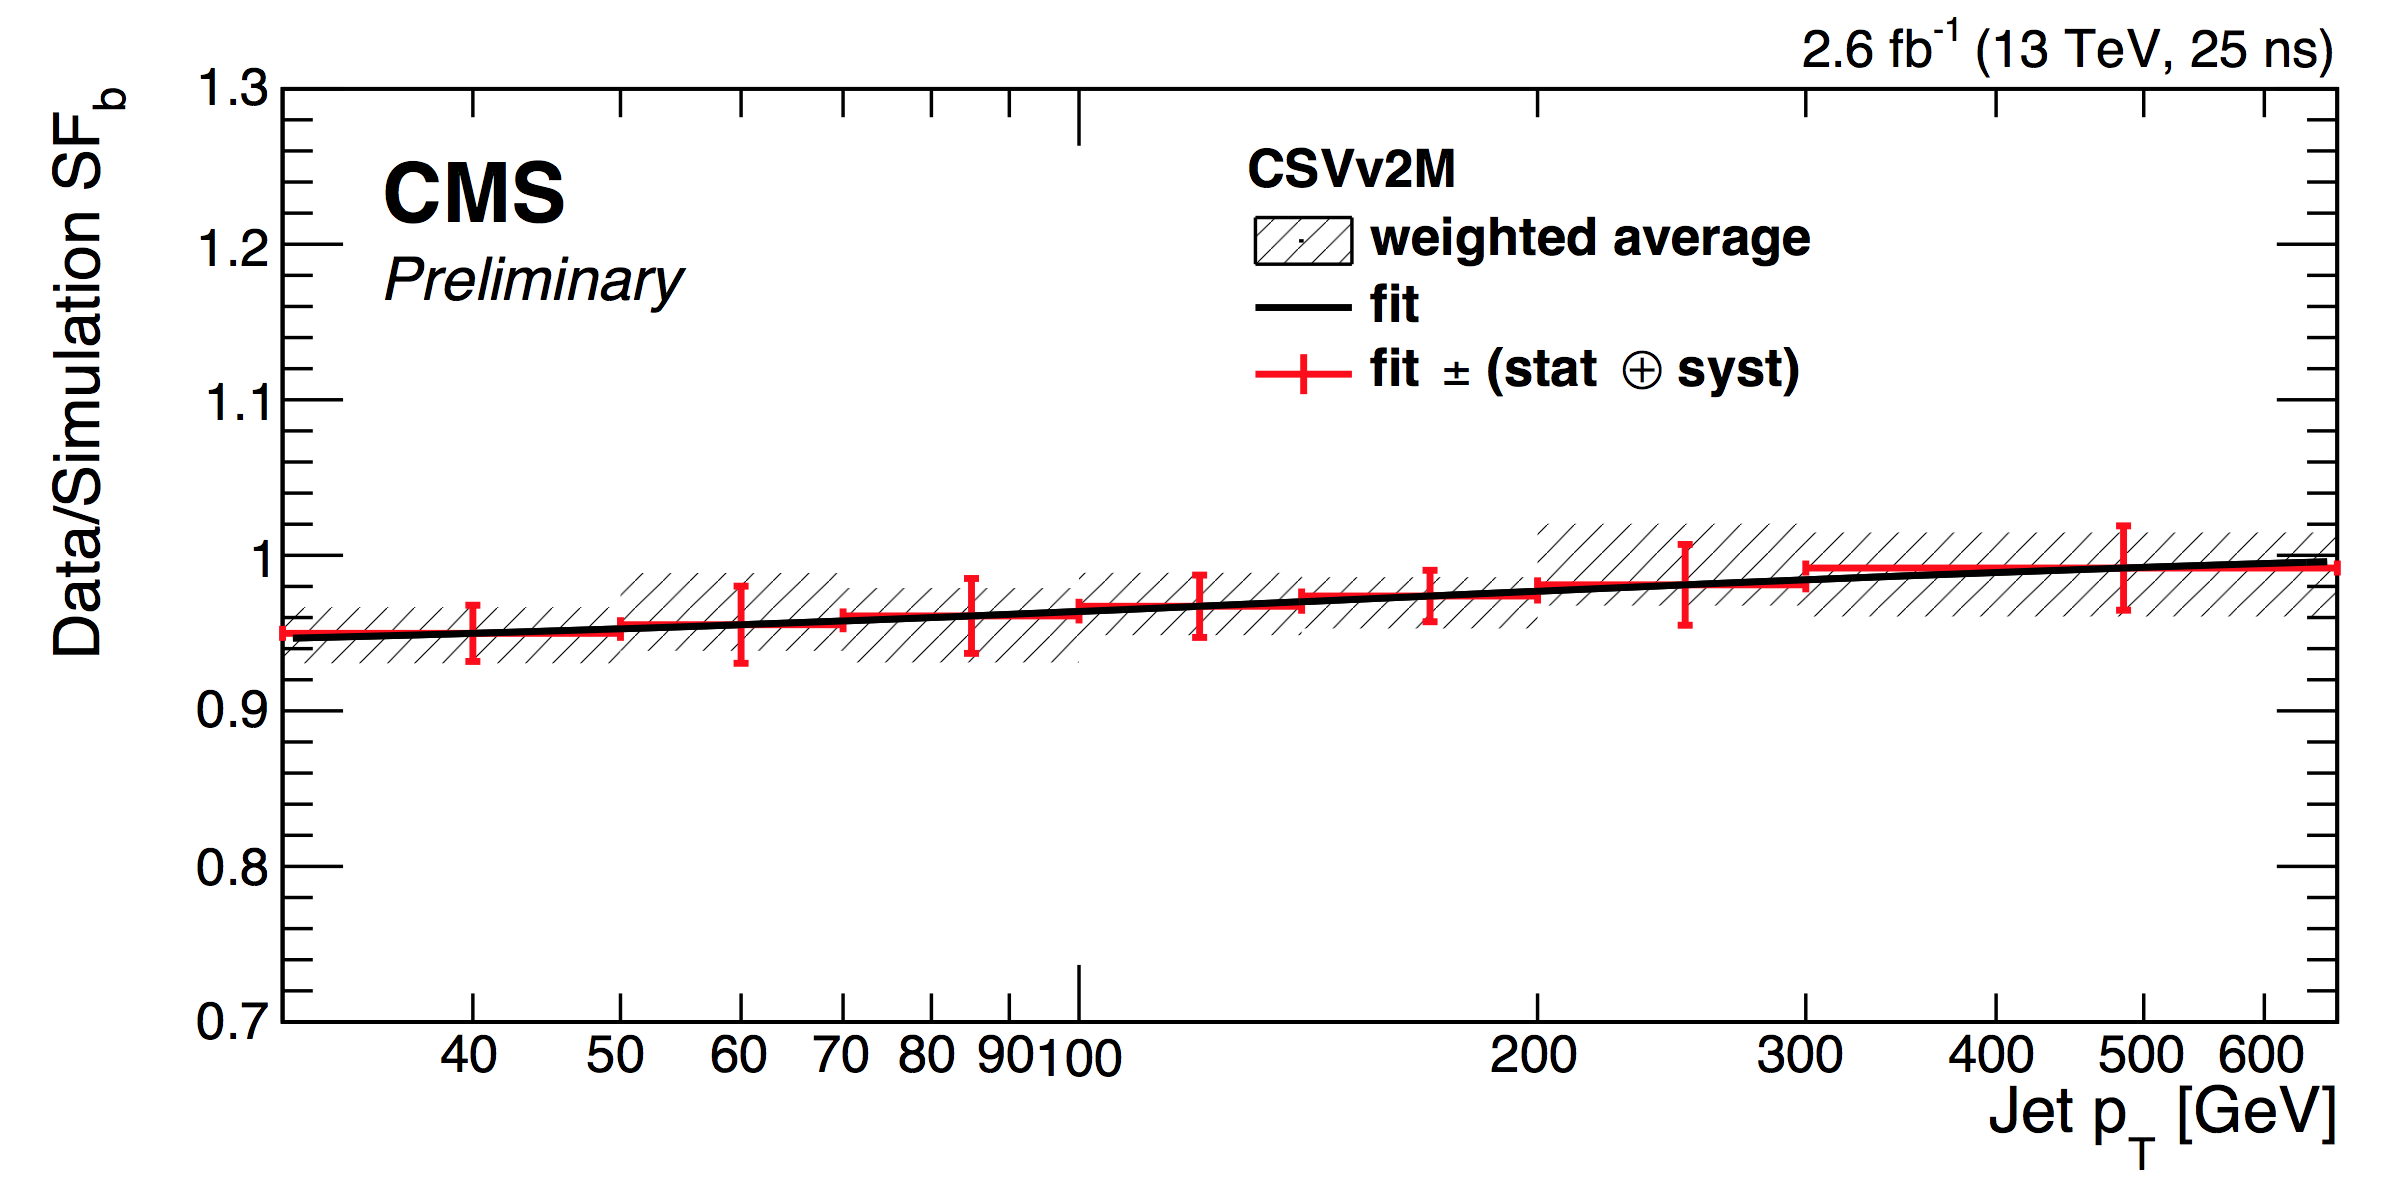
\includegraphics[width=0.7\textwidth]{./Objects/Plots/CSVSF.png}
\caption[The b-tagging scale factors and uncertainties for b-jets in the data sample collected during 2015 as a function of jet \pT~for the medium working point of the CSVv2 discriminant.]{%(a) distribution of CSVv2 discriminant for multijet events in $2.6\,\invfb$ 
%collected at $\sqrt{s} = 13$ TeV and (b) 
The b-tagging scale factors and uncertainties for b-jets in the data sample collected during 2015
as a function of jet \pT~for the medium working point of the CSVv2 discriminant \cite{cms-btag-run2}.}
\label{fig:objects_bjets}
\end{figure}

Systematic uncertainties in the scale factors arise from, amongst other things,
pileup modelling in simulation, gluon splitting into $\Pbottom\APbottom$ pairs, track mismeasurement,
and uncertainties in the fractions of different jet types.
Figure \ref{fig:objects_bjets} shows the b-tagging scale factors, and associated uncertainties,
for the medium working point of the \ac{CSV}v2 discriminator in the
2015 data sample.
%Some efficiency measurements are performed using samples that include a jet with a muon within ∆R = 0.4 from the jet axis (a “muon jet”). Because the semileptonic branching fraction of b hadrons is significantly larger than that for other hadrons (about 11%, or 20% when b → c → l cascade decays are included), these jets are more likely to arise from b quarks than from another flavour.
%The combinatorial complexity of the reconstruction of the decay points (secondary vertices) of b or c hadrons is more challenging in the presence of multiple proton-proton interactions. In order to minimize this complexity a different track selection is applied. Tracks must be within a cone of ∆R = 0.3 around the jet axis with a maximal distance to this axis of 0.2 cm and pass a “high-purity” criterion [32]. The “high-purity” criterion uses the normalized χ2 of the track fit, the track length, and impact parameter information to optimize the purity for each of the iterations in track reconstruction. The vertex finding procedure begins with tracks defined by this selection and proceeds iteratively. A vertex candidate is identified by applying an adaptive vertex fit [31], which is robust in the presence of outliers. The fit estimates the vertex position and assigns a weight between 0 and 1 to each track based on its compatibility with the vertex. All tracks with weights > 0.5 are then removed from the sample. The fit procedure is repeated until no new vertex candidate can be found. In the first iteration the interaction region is used as a constraint in order to identify the prompt tracks in the jet. The subsequent iterations produce decay vertex candidates.

\section{Missing energy}
\label{sec:objects_met}
The \ac{CMS} detector is able to detect most stable and long-lived particles,
however, neutrinos and hypothetical neutral weakly interacting particles
travel straight through the detector without being recorded. These particles
will give rise to an energy imbalance in the transverse plane, and so their
presence can be inferred from missing transverse energy, \MET, in the event. 

The \MET~is defined as $-\Sigma \vec{p}_{\text{T}}$, where
the sum runs over all final-state particles and jets in the event. This quantity
can be mismeasured due to detector inefficiencies, calorimeter energy thresholds and
the nonlinearity of the calorimeter
response for hadronic particles.
Therefore, to increase the accuracy of the \MET~measurement the jet energy corrections are propagated as
\begin{equation}\label{eqn:objects_met_corr}
\vec{E}_{\text{T}}^{\text{miss, corr}} = \vec{E}_{\text{T}}^{\text{miss}} - \Sigma_{jets} (\vec{p}_{\text{T,jet}}^{\text{  corr}} - \vec{p}_{\text{T,jet}}),
\end{equation}
where `corr' refers to the corrected values.
%The magnitude of the ⃗E/T can be underestimated or overestimated for a variety of reasons, including minimum energy thresholds in the calorimeters, pT thresholds and inefficiencies in the tracker, and the nonlinearity of the response of the calorimeter for hadronic particles due to its non-compensating nature. This bias is significantly reduced by correcting the pT of jets to the particle-level pT using jet energy corrections 
The \MET~can also be mismeasured due to pileup interactions, and an improved
measurement of the \MET~at high pileup can be obtained by using the MVA \MET~
algorithm, used for \MET~reconstruction in the \Htohhtobbtautau and \AHtotautau analyses.
This algorithm computes a correction to the hadronic
recoil $\vec{u}_{\text{T}}$ reconstructed from \ac{PF} particles
\begin{equation}\label{eqn:objects_met_recoil}
\vec{u}_{\text{T}} = \vec{E}_{\text{T}}^{\text{miss}} - \Sigma \vec{p}_{\text{T}}^{\text{  lep}},
\end{equation}
where $\Sigma \vec{p}_{\text{T}}^{\text{  lep}}$ corresponds to the vectorial sum of the transverse momenta of the
constituents selected as the di-tau candidate.

Two \acp{BDT} trained on \Zmm events are used to compute this correction.
The first one corrects the direction of the hadronic recoil, and the second
one uses a data sample with the corrected recoil direction to compute a correction
to the magnitude of the hadronic recoil. This \ac{BDT} regression uses the magnitude of the hadronic
recoil, its azimuthal angle and the scalar \pT~sum of all \ac{PF} particles for several 
different \MET~definitions \cite{cms-met-run1} as input. Figure \ref{fig:objects_mvamet} shows
the performance of the MVA \MET~in data collected at $\sqrt{s}=13\,\TeV$ compared with 
the \ac{PF} \MET. Figure \ref{fig:objects_mvamet}a indicates the lower MVA \MET~values for events without genuine
\MET and figure \ref{fig:objects_mvamet}b shows the improved resolution at high pileup.

In the process of calculating the corrections to the hadronic recoil using the MVA \MET~algorithm, an event-by-event
estimator of the likelihood that the \MET~is due to unseen objects rather than induced
by mismeasurement of jet energy is also determined~\cite{cms-met-run1}.

\begin{figure}[h!]
\begin{center}
\subfloat[\MET~distribution in \Zmm events]{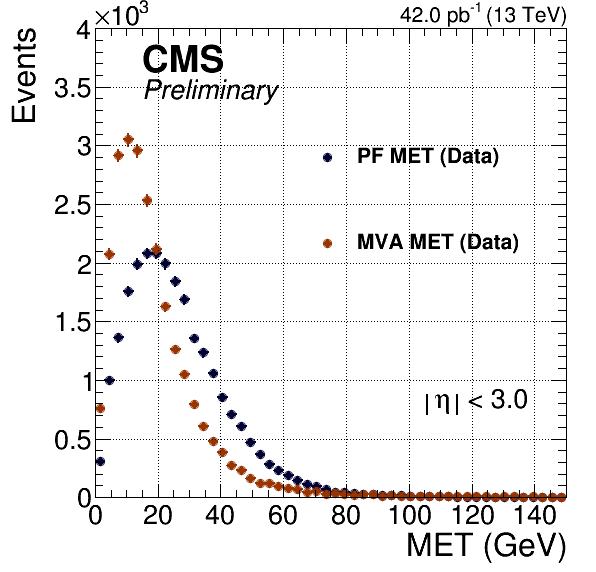
\includegraphics[width=0.5\textwidth]{./Objects/Plots/Met_Data.png}}
\subfloat[\MET~resolution]{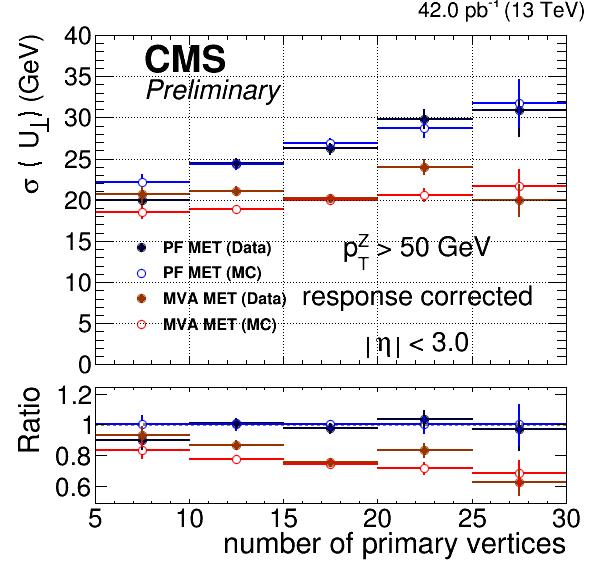
\includegraphics[width=0.5\textwidth]{./Objects/Plots/transverse_resolution_npv.png}}
\end{center}
\caption[\MET~distributions comparing MVA \MET~to PF \MET~for
\Zmm events, in a sample corresponding to $42\,\invpb$ of data collected
at \mbox{$\sqrt{s}=13\,\TeV$}.]{(a) \MET~distributions comparing MVA \MET~(brown circles) to \ac{PF} \MET~(black circles) for
\Zmm events, which contain no genuine \MET~, in a sample corresponding to $42\,\invpb$ of data collected at $\sqrt{s}=13\,\TeV$. The 
\MET~values for MVA \MET~are lower than for \ac{PF} \MET. (b) The \MET~resolution for \ac{PF} \MET~in blue and MVA \MET~in red/brown
circles, as a function of number of vertices. The MVA \MET~resolution is more stable with increased pileup \cite{cms-dp-mvamet}.}
\label{fig:objects_mvamet}
\end{figure}


%Further corrections improve the performance of the ⃗E/T reconstruction in events with large numbers of pileup interactions. The contribution to the genuine ⃗E/T from such interactions is
%close to zero, as the probability to produce neutrinos is small in inelastic pp scattering (mini- mum bias) interactions. The vectorial ⃗pT sum of charged particles is therefore expected to be well balanced by that of neutral particles. However, the nonlinearity and minimum energy thresholds in the calorimeters cause ⃗E/ T to point on average in the direction of the vectorial ⃗pT sum of neutral particles.

\subsection{Recoil corrections}
\label{sec:objects_met_recoilcorr}
To correct for the mis-modelling of \MET~in simulated events, recoil corrections are determined. 
The hadronic recoil $\vec{u}_{\text{T}} = \vec{E}_{\text{T}}^{\text{miss}} - \Sigma \vec{p}_{\text{T}}^{\text{ leptons}/\nu}$ 
is projected onto the axes parallel, $u_{\parallel}$, and perpendicular, $u_{\perp}$, to the \pT~of the boson producing the leptons
and neutrinos. For the \Htohhtobbtautau and \AHtotautau analyses 
it is measured in \Zmm events, where no neutrinos
are present. Distributions of $u_{\parallel}$ and $u_{\perp}$ are fitted both in data
and simulated events, using convolutions of gaussians. Corrections are then applied to the simulation
as
\begin{equation}\label{eqn:met_recoilcorr}
u_{\parallel,\perp}' = <u_{\parallel,\perp}>_{\text{data}} + (u_{\parallel,\perp} - <u_{\parallel,\perp}>_{\text{MC}}) \cdot \frac{\sigma_{\text{Data}}}{\sigma_{\text{MC}}}.
\end{equation}
%Recoil corrections are applied to correct for the mismodelling of $\MET$ in events without genuine $\MET$ \cite{RecoilCorrPresentation}.
%The hadronic recoil is defined as
%$\vec{U} = \vec{E}_{\text{T}}^{mis} - \Sigma \vec{p}_{\text{T},\nu/lep}$. This recoil is projected onto the axes parallel ($U_1$) and
%orthogonal ($U_2$) to the boson $p_{\text{T}}$ and it is measured in $Z\rightarrow\mu\mu$ events, in which the $\nu$ term is 0. Events are selected
%by requiring the HLT\_IsoMu22\_v trigger in data, and opposite--sign muon pairs are selected by requiring two muons with opposite charge, passing
%the medium HIP safe muon ID, the same impact parameter cuts as in the muon selection for the analysis, $I_{rel}^{\mu} < 0.15$. The leading
%muon must have a $p_{\text{T}}$ of at least 23 GeV, with the trailing muon having a $p_{\text{T}}$ of at least 10 GeV. In addition, for data
%events the leading muon must have fired the HLT\_IsoMu22\_v trigger. The requirements on muon $\eta$ are $|\eta_1| < 2.1$ and $|\eta_2|<2.4$.
%At pair level, the two muons must be separated by $\Delta R > 0.5$, and the di-muon mass must be at least 20 GeV. Pile--up reweighting,
%the muon ID, isolation, and trigger scale factors are applied, as are the muon tracking efficiencies. The DY shape reweighting
%is applied to DY MC and top $p_{T}$ reweighting is applied to the $t\bar{t}$ MC.
%The projected hadronic recoil $U$
%is determined for both $Z\rightarrow\mu\mu$ data and MC events. A double gaussian with means symmetrically shifted away from zero is used to fit the $U_2$ component,
%with a triple  gaussians for fitting the $U_1$ component. These fits are performed in bins of $Z p_{\text{T}}$ (0-10, 10-20, 20-30, 30-50, and $ > 50$ GeV), and
%bins of number of jets (0, 1 or at least 2). $Z\rightarrow \mu\mu$ events from around the Z peak are used by requiring $70 <m_{\mu\mu} < 110 $ GeV.
%To apply the corrections, the offset $w = U{1,2} -<U_{1,2}>_{MC} $ and the recoil in MC is corrected as
%$U_{1,2}' = <U_{1,2}>_{data} + w\frac{\sigma_{data}}{\sigma_{MC}}$.

\section{Hadronic taus}
\label{sec:objects_tau}
Taus are unstable particles and they decay before reaching the detector. In 17.4\% of 
cases they decay to muons and neutrinos, with an additional 17.8\% decaying to electrons
plus neutrinos. The remaining 64.8\% decay hadronically. Hadronically decaying
taus, \Pgth, are characterised by narrow jets containing either one or three charged
particles ($\pi^{\pm}, K^{\pm}$) and zero, one, or two neutral pions. An overview
of the most common decay modes is given in table \ref{tab:hadronic_tau_decays}.
\begin{table}[htp]
\begin{center}
\caption[Summary of hadronic tau decay modes.]{Summary of hadronic tau decay modes, indicating the branching fraction, and intermediate resonances where relevant \cite{pdg-2014}.}
\begin{tabular}{@{}lll@{}}
%\toprule
\textbf{Decay mode} & \textbf{Resonance} &\textbf{Branching fraction [\%]}\\
\midrule
\Ptaupm $\rightarrow$ h$^{\pm}$\Pnut & & 11.5\%\\
\Ptaupm $\rightarrow$ h$^{\pm}$\Ppizero\Pnut& $\rho$(770) & 26.0\% \\
\Ptaupm $\rightarrow$ h$^{\pm}$\Ppizero\Ppizero\Pnut & a$_{1}$(1260) & 9.5\% \\
\Ptaupm $\rightarrow$ h$^{\pm}$h$^{\mp}$h$^{\pm}$\Pnut & a$_{1}$(1260) & 9.8\% \\
\Ptaupm $\rightarrow$ h$^{\pm}$h$^{\mp}$h$^{\pm}$\Ppizero\Pnut & & 4.8\%\\
Other modes with hadrons & & 3.2\% \\
\midrule
Total & & 64.8\% \\
%\bottomrule
\end{tabular}
\label{tab:hadronic_tau_decays}
\end{center}
\end{table}
%\subsection{Identification}
%\label{sec:objects_tau_id}

Hadronic tau decays are reconstructed using the ``hadrons plus strips'' (HPS) algorithm~\cite{cms-tau-run1,cms-tau-2015}, 
which is seeded by jets clustered from \ac{PF} candidates, using the anti-\kT~algorithm with a distance parameter $\Delta R = 0.5$ in
Run~1 and $\Delta R = 0.4$ in Run~2. 
As table \ref{tab:hadronic_tau_decays}
shows, 62\% of hadronic tau decays contain at least one \Ppizero in the final state. There is a large
probability that photons from $\Ppizero \rightarrow \Pphoton \Pphoton$ decays will convert to
$\APelectron \Pelectron$ pairs, which are bent in the magnetic field and 
therefore cause showers dispersed in the $\phi$ direction in the \ac{ECAL}. Therefore, to 
reconstruct the energy deposits \Ppizero candidates leave in the ECAL, 
the photon and electron constituents of the jet that seeds the \Pgth reconstruction are clustered into strips.
The electron or photon with the highest \pT~that is not yet included in a strip is used to build a new strip.
The $\eta$ and $\phi$ of this candidate determine the initial position of the strip, the next highest \pT~electron or photon
within an $\eta \times \phi$ window centered on the strip location is added to the strip and the position is 
recomputed as the energy-weighted average of the electron and photon constituents in the strip.
This procedure is repeated until there are no more electrons or photons with \pT~$ > 0.5\,\GeV$ within the 
strip window. During Run~1 the strip window had a fixed size of $0.05 \times 0.2$ in $\eta \times \phi$, 
while in the algorithm used during Run~2 the strip size is dynamically allocated. The
width of the strip in $\eta$ and $\phi$ is varied based on the \pT~or \ET~to 
be added to the strip and on the energy the strip already has, as
\begin{equation}\label{eqn:dynamicstrip}
\begin{split}
&\Delta \eta  = 0.2\cdot p_{\text{T},\Pe/\Pphoton}^{-0.66} + 0.2\cdot p_{\text{T,strip}}^{-0.66} \\
&\Delta \phi  = 0.35\cdot p_{\text{T},\Pe/\Pphoton}^{-0.71} + 0.35\cdot p_{\text{T,strip}}^{-0.71},\\
\end{split}
\end{equation}
where $p_{\text{T},\Pe/\Pphoton}$ is the transverse momentum of the candidate to be added to the strip
and $p_{\text{T,strip}}$ is the transverse momentum of the strip before merging a new candidate in.\\%FIXME EXPLAIN WHERE THIS COMES FROM SEE AN ETC
In addition, the strip size is bounded as $0.05 < \Delta\eta < 0.15$ and $0.05 < \Delta\phi < 0.3$ \cite{cms-tau-2015}.

%The functions $f(p_{\text{T}})$ and $g(p_{\text{T}})$ are defined as:
%\begin{equation}\label{eqn:dynamicstripfg}
%\begin{split}
%&f(p_{\text{T}}) = 0.2\cdot p_{\text{T}}^{-0.66} \text{ and } \\
%&g(p_{\text{T}}) = 0.35\cdot p_{\text{T}}^{-0.71}.\\
%\end{split}
%\end{equation}
If the $\Sigma$ \pT~of the strip is at least $2.5\,\GeV$ it is considered as a \Ppizero candidate.
To reconstruct hadronic taus, charged particles and strips are combined into different signatures which are said to be
compatible with a certain decay mode if the selection listed below is satisfied. The charged particles
and strips are required to be within the signal cone $R_{\text{sig}} = \frac{3.0}{p_{\text{T}}[\GeV]}$, bounded 
by $0.05 < R_{\text{sig}} < 0.1$.
If a candidate satisfies more than one of the hypotheses the one that maximises the \pT~is retained.
The decay modes considered for reconstructing hadronic taus are:
\begin{itemize}
\setlength{\itemsep}{-0.5\baselineskip}
\item \textbf{One prong + 0 \Ppizero :} One charged particle, no strips.
\item \textbf{One prong + 1 \Ppizero :} One charged particle and one strip with tau mass requirement $ 0.3 < m_{\Pgt} < 1.3 \sqrt{p_{\text{T}}/100}\,\GeV$, with this
upper limit on the mass at least $1.3\,\GeV$ and at most $4.2\,\GeV$.
%less than 100 GeV, the upper limit is fixed to 1.3 GeV, and for momenta larger than 1044 GeV the upper limit on $m_{\Pgt}$ is fixed to 4.2 GeV.
\item \textbf{One prong + 2 \Ppizero :} One charged particle and two strips. The tau mass should be $0.4 < m_{\Pgt} < 1.2\sqrt{p_{\text{T}}/100}\,\GeV$, with the
upper limit on the mass at least $1.2\,\GeV$ and at most $4.0\,\GeV$.
%less than 100 GeV, the upper limit is fixed to 1.2 GeV and for momenta larger than 1111 GeV the upper limit on $m_{\Pgt}$ is fixed to 4.0 GeV.
\item \textbf{Three prong + 0 \Ppizero: } Three charged particles with mass $0.8 < m_{\tau} < 1.5\,\GeV$. The tracks are required to originate 
within $\Delta z<0.4$~cm of the same vertex, and their total charge is required to be $\pm 1$.
\end{itemize}

%\subsection{Isolation and discrimination against light leptons}
%\label{sec:objects_tau_iso}
Requiring the reconstructed \Pgth to be isolated reduces the $\text{jet}\rightarrow\Pgth$ fake rate. Isolation
discriminators can be defined using the isolation sum,
\begin{equation}\label{eqn:cutbased_iso}
I_{\Pgt} = \Sigma p_{\text{T}}^{\text{charged}}(d_Z < 0.2\text{ cm}) + \text{max}(0,\Sigma p_{\text{T}}^{\Pphoton} - \Delta \beta \Sigma p_{\text{T}}^{\text{charged}} (d_Z > 0.2 \text{ cm}) ),
\end{equation}
where the first term denotes the sum of the transverse momenta of all charged particles not part
of the identified \Pgth. Only particles with \pT~$> 0.5\,\GeV$ within a cone of $\Delta R = 0.5$ centred around the 
direction of the \Pgth are taken into account and the charged particle tracks are required to be compatible with having
originated from the \Pgth production vertex. This is achieved by requiring the longitudinal impact parameter
with respect to the primary vertex to be $d_z < 0.2\,\cm$. The second term of equation \ref{eqn:cutbased_iso} denotes the sum
of the transverse momenta of photons with $\pTm > 0.5$ GeV within a cone of $\Delta R = 0.5$ centred around the direction
of the \Pgth. The effect of pileup on this term is accounted for by subtracting the sum of the momenta of charged
particles with \pT~$> 0.5\,\GeV$, within a cone of $\Delta R = 0.8$ around the direction of the hadronic tau and
tracks not compatible with having originated from the production vertex of the hadronic tau, multiplied by
a $\Delta \beta$ factor of 0.2.%FIXME rephrase

In addition to the isolation sum, a requirement on the sum of transverse momenta
of electrons and photons included in strips but which are located outside of the signal cone,
\begin{equation}\label{eqn:ptouter_iso}
p_{\text{T}}^{\text{strip, outer}} = \Sigma p_{\text{T}}^{\Pe/\Pphoton}(\Delta R > R_{\text{sig}}) < 0.10\cdot p_{\text{T}}^{\Pgt},
\end{equation}
can be made.
An MVA \Pgth isolation discriminator combines isolation variables with tau lifetime information into a \ac{BDT} to discriminate between \Pgth decays and quark and gluon jets.
Some of the variables used as input are:
\begin{itemize}
\setlength{\itemsep}{-0.5\baselineskip}
\item Isolation sums, including those in equations \ref{eqn:cutbased_iso} and \ref{eqn:ptouter_iso}.
\item Track-related variables such as impact parameters, quality of the track, and information about decay vertices.
\item Information about photons: the momentum-weighted $\Delta R$, $\Delta \eta$ and $\Delta \phi$ of photons in strips inside or outside the signal cone, in addition to the number of signal and isolation photons found.
\item \Pgth-related kinematic quantities, plus the reconstructed decay mode.  
%\item The charged-and neutral-particle isolation sums
%\item The reconstructed $\tau_{h}$ decay mode
%\item The transverse impact parameter $d_{xy}$ of the leading track of the $\tau_{h}$ candidate with the vertex, and its significance $d_{xy}/\sigma_{d_{xy}}$, and its sign (the projection of the impact parameter vector on the $\tau_h$ direction)
%\item The 3-dimensional impact parameter $d_{xyz}$ of the leading track, and it significance
%\item The distance between the $\tau$ production and decay vertices, its significance, and information about whether a decay vertex has successfully been reconstructed for a given candidate.
%\item $p_{\text{T}}$ and $\eta$ of the $\tau_{h}$ candidate
%\item $\Delta \beta$ corrected isolation (as equation \ref{eqn:cutbased_iso}
%\item The sum of transverse momenta of electrons and photons included in strips but located outside of the signal cone (equation \ref{eqn:ptouter_iso})
%\item The $\chi^2$ value of the fit for the leading track of the $\tau_{h}$ candidate
%\item The ratio of the total electromagnetic energy to the total energy within the $\tau_h$ signal cone.
%\item The total number of signal and isolation photons with $p_{\text{T}} > 0.5$~GeV
%\item The $p_{\text{T}}$ weighted $\Delta R$ of photons within signal cone and the isolation annulus
%\item The $p_{\text{T}}$ weighted $\Delta \eta$ and $\Delta \phi$ of photons in strips outside of the signal cone.
\end{itemize}

Figure \ref{fig:tau_efficiency}a compares the \Pgth identification efficiency with the
$\text{jet}\rightarrow\Pgth$ fake rate for different working points of the
MVA isolation discriminator, as well as the cut-based isolation discriminator based
on the isolation sum and $p_{\text{T}}^{\text{strip,outer}}$. The MVA-based 
discriminator performs better than the cut-based discriminator alone.

In order to reduce the $\Pe\rightarrow\Pgth$ and $\Pgm\rightarrow\Pgth$ fake rates, 
anti-electron and anti-muon discriminators are used. 
The anti-electron discriminator is a \ac{BDT}-based discriminator trained using input variables such as:
\begin{itemize}
\setlength{\itemsep}{-0.5\baselineskip}
\item Kinematic variables of the \Pgth candidate and \ac{GSF} track, including visible mass of the \Pgth.
\item Energy and momentum ratios such as the fraction of electromagnetic energy, \ac{ECAL} and \ac{HCAL} energy relative to track momentum.
\item Photon-related variables, such as the momentum-weighted $\Delta \eta$ and $\Delta \phi$ between photons, the fraction of the \Pgth energy carried by photons, and the number of photons found in strips.
\item Information on the quality of the track.
%\item \pT, $\eta$ of the $\Pgt_{h}$ candidate
%\item \pT, $\eta$, $\sigma_{p_{\text{T}}}/p_{\text{T}}$ of the \ac{GSF} track
%\item Distance in $\eta$ and $\phi$ of the \ac{GSF} track to the nearest boundary between \ac{ECAL} modules.
%\item Electromagnetic energy fraction $E_{\text{ECAL}}/(E_{\text{ECAL}}+E_{\text{HCAL}})$
%\item Ratio of \ac{ECAL} and \ac{HCAL} energy fractions relative to the momentum of the leading charged track
%\item The \pT weighted RMS distances in $\eta$ and $\phi$ between the photons in any strip and the leading 
%charged track (calculated separately for photons inside and outside the $\Pgt$ signal cone)
%\item The fraction of $\Pgt_{h}$ energy carried by photons (calculated separately for photons inside and outside the $\Pgt_h$ signal cone)
%\item $(p_{in} - p_{out})/p_{in}$
%\item The number of photons in any of the strips associated with the $\Pgt_h$ candidate, calculated separately for photons inside and outside the $\Pgt_h$ signal cone
%\item The ratio between the total \ac{ECAL} energy and inner track momentum
%\item The ratio of energies of bremsstrahlung photons measured in the \ac{ECAL} and the tracker
%\item The visible mass of the $\Pgt_h$ candidate, for photons and charged particles within the $\Pgt_h$ signal cone
%\item $\chi^2/Ndof$ of the GSF track fit
%\item $N_{hits}^{GSF}-N_{hits}^{KF}/N_{hits}^{GSF}+N_{hits}^{KF}$, With $N_{hits}^{GSF}$ the number of hits associated with the track in the \ac{GSF} track reconstruction algorithm, and
%similarly $N_{hits}^{KF}$ for the \ac{KF} track reconstruction algorithm.
\end{itemize}

Five working points are provided, ranging from very loose to very tight. The \Pgth efficiency
and $\Pe\rightarrow$\Pgth fake rate for the various working points are shown in
figures \ref{fig:tau_efficiency}b and \ref{fig:tau_efficiency}c, respectively.

\begin{figure}[h!]
\begin{center}
\subfloat[Isolation performance]{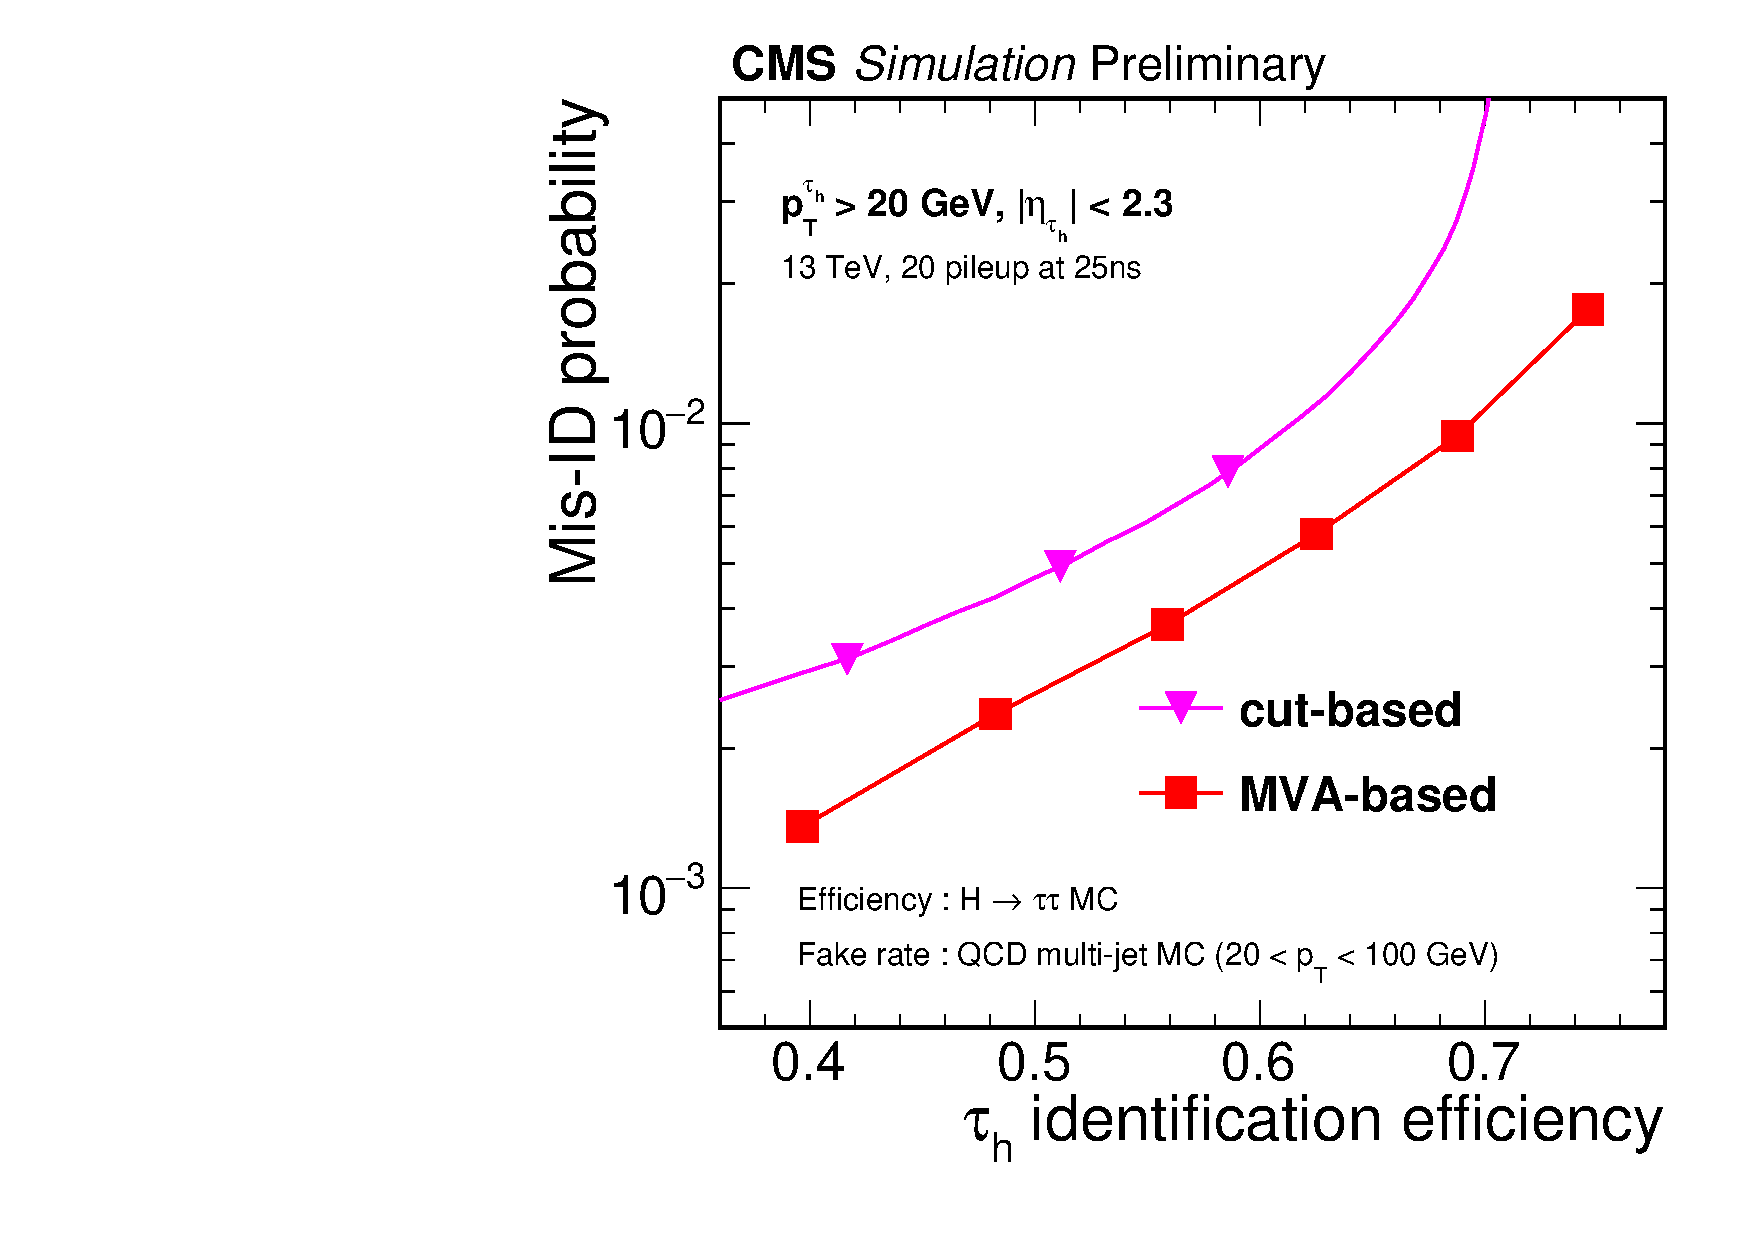
\includegraphics[width=0.5\textwidth]{./Objects/Plots/TauEfficiencyIsol.pdf}}\\
\subfloat[Real \Pgth efficiency for anti-\Pe discriminator]{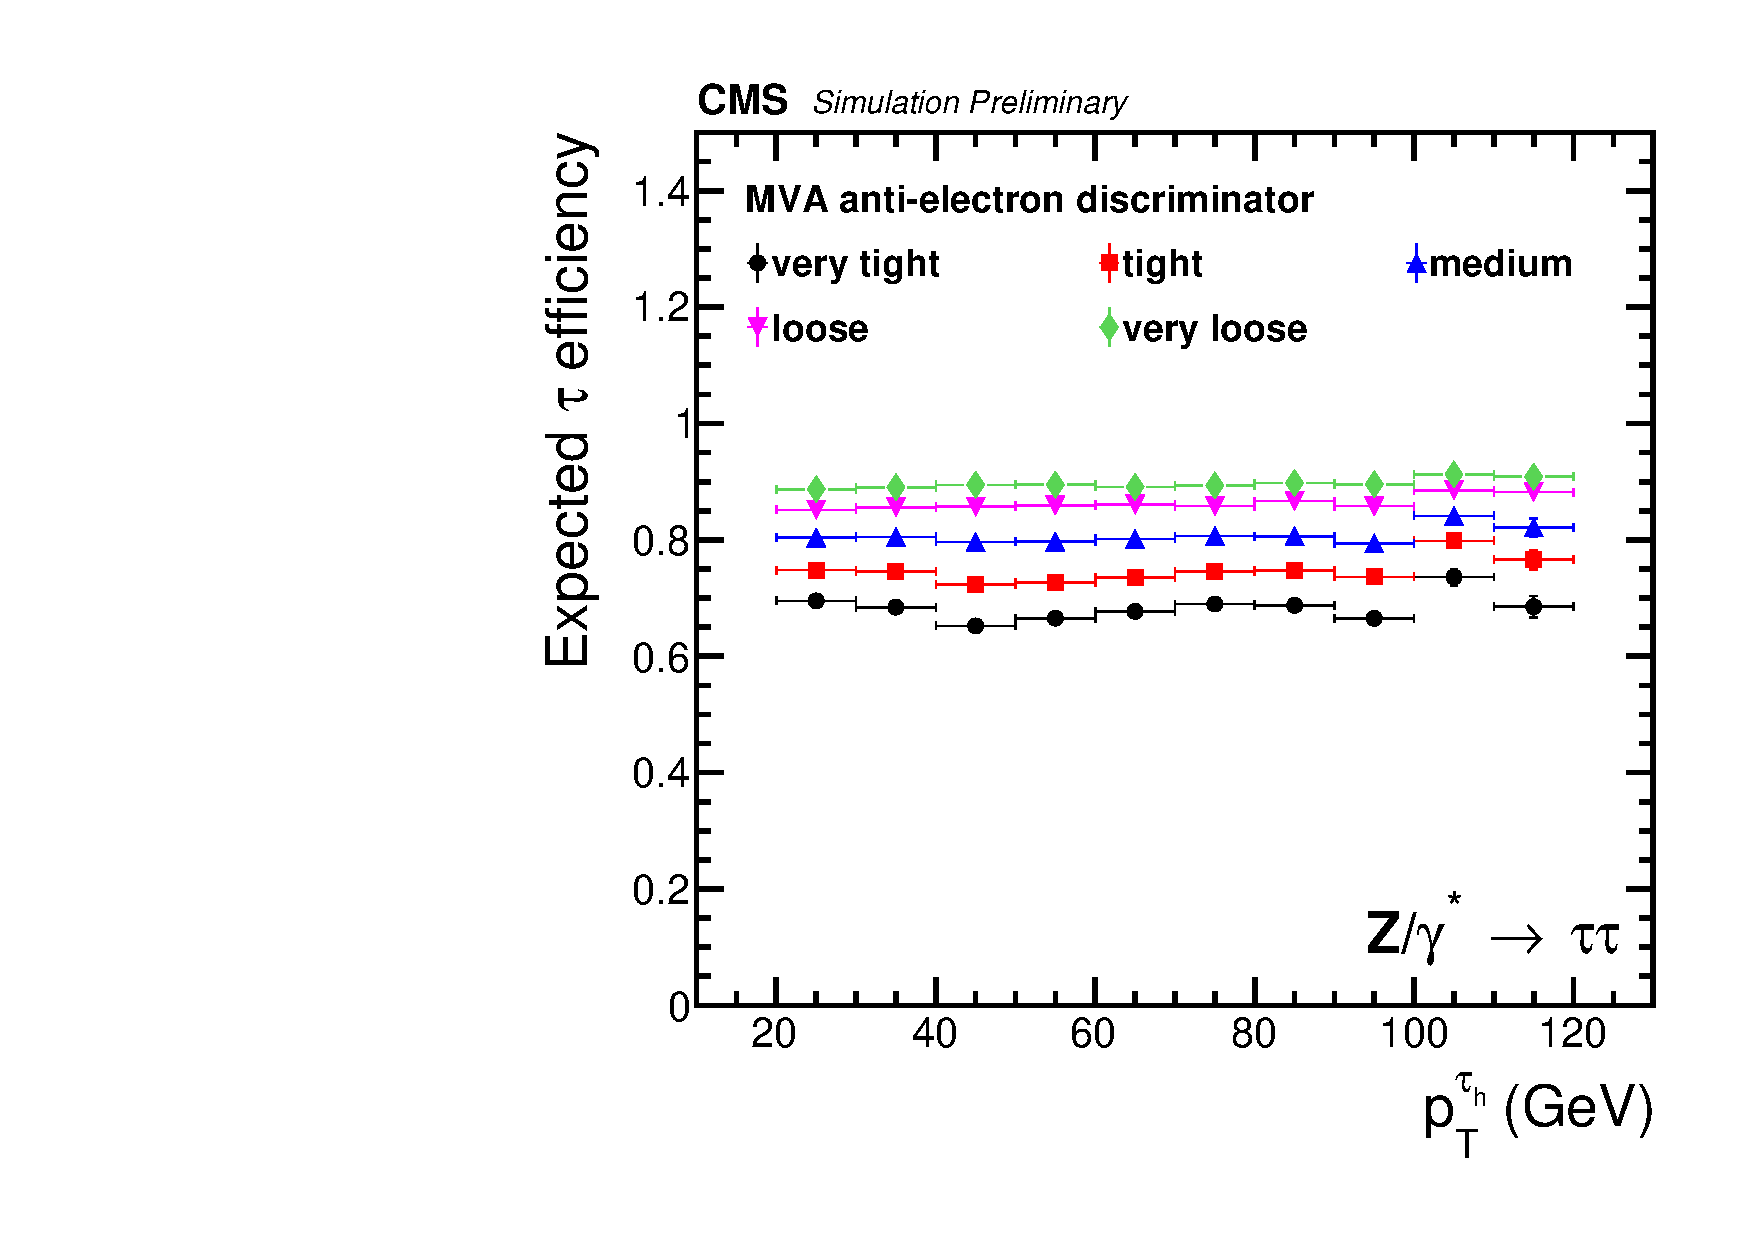
\includegraphics[width=0.5\textwidth]{./Objects/Plots/TauEfficiencyEle.pdf}}
\subfloat[$\Pe\rightarrow$\Pgth fake rate for the anti-\Pe discriminator]{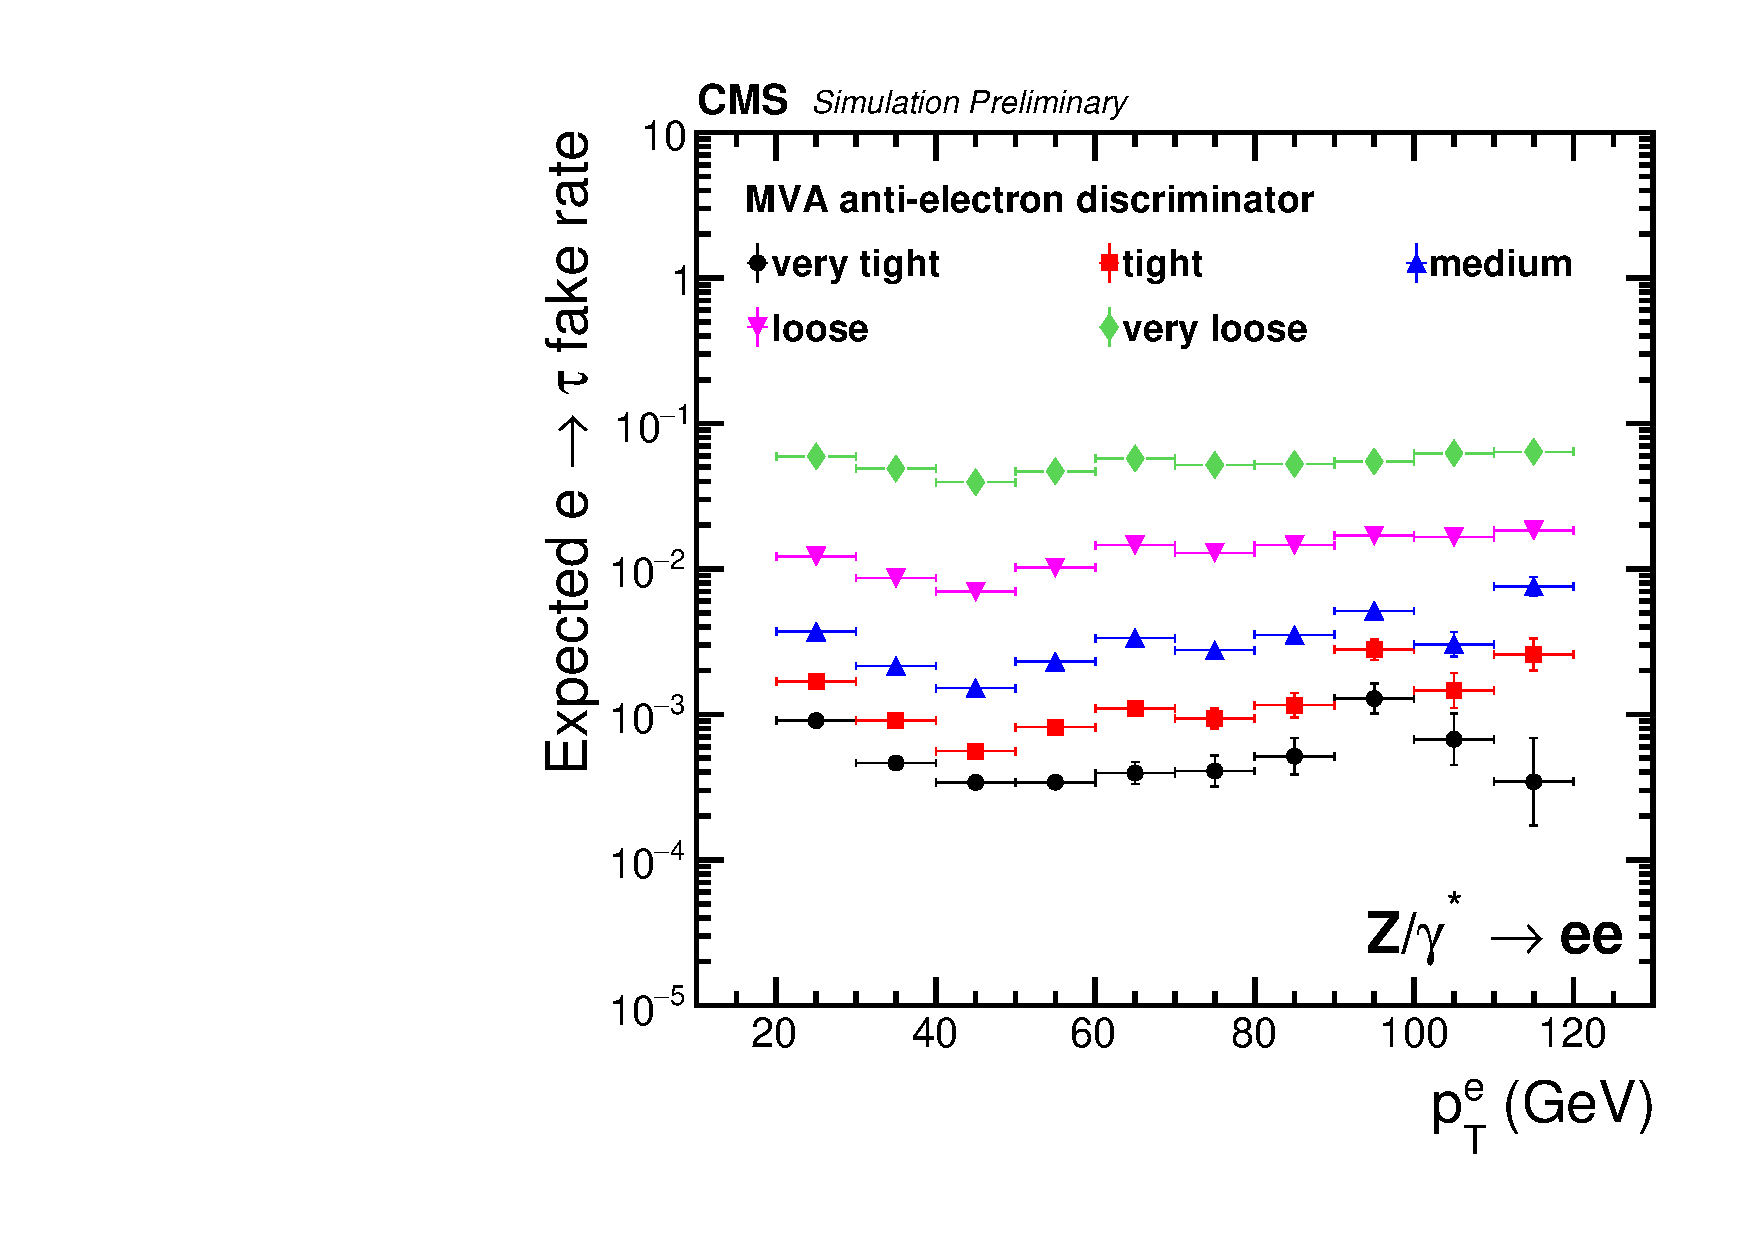
\includegraphics[width=0.5\textwidth]{./Objects/Plots/TauMisIDEle.pdf}}
\end{center}
\caption[Figures of the jet$\rightarrow$\Pgth fake rate in simulated QCD events
versus $\Pgth$ identification efficiency for simulated $\PHiggs\rightarrow\Pgt\Pgt$ events, the real
$\Pgth$ identification efficiency for different working points of the anti-electron discriminator, and the \mbox{$\Pe\rightarrow\Pgth$} fake rate for different
working points of the anti-electron discriminator.]{(a) The jet$\rightarrow$\Pgth fake rate in simulated QCD multijet events versus \Pgth identification
efficiency for simulated $\PHiggs\rightarrow\Pgt\Pgt$ events, comparing the MVA-based isolation discriminator in red with the cut-based 
isolation discriminator in pink. Tighter working points give lower hadronic tau identification
efficiencies and lower fake rates, and for the same \Pgth identification efficiency the fake rate
from the MVA-based discriminator is lower than from the cut-based discriminator. (b) The real \Pgth identification
efficiency for different working points of the anti-electron discriminator as a function of the \pT~of the \Pgth, and (c)
the $\Pe\rightarrow$\Pgth fake rate for different working points of the anti-electron discriminator, as a function of
the \pT~of the electron \cite{cms-tau-2015}.}
\label{fig:tau_efficiency}
\end{figure}
The anti-muon discriminator is a cut-based discriminant, for which a loose and a tight working
point are provided. It is based on variables such as the number of track segments found in various
parts of the muon system around the direction of the \Pgth, and comparisons of calorimeter energy
with the momentum of the leading \Pgth track.
%\begin{itemize}
%\setlength{\itemsep}{-\baselineskip}
%\item \textbf{Loose:} The $\Pgt_h$ candidate is vetoed by this discriminator if track segments are found in at least two muon stations within a cone of $\Delta R = 0.3$ of the $\Pgt_h$ direction, or if the sum of the electromagnetic and hadronic energy ($E_{\text{ECAL}}+E_{\text{HCAL}}$) is smaller than $0.2\cdot p_{\text{leading track}}$.
%Otherwise it passes the discriminator.
%\item \textbf{Tight:} The $\Pgt_h$ candidate passes this working point if it passes the loose working point and no hits are present within a cone of $\Delta R=0.3$ of the $\Pgt_h$ direction in the \ac{CSCs},\ac{RPCs} and \ac{DT} in the two outermost muon stations.
%\end{itemize}

